% !TeX program = xelatex
% --- 1. FONT SIZE: 11pt (Strictly per Template) ---
\documentclass[11pt,a4paper]{report}

% =========================================================
% 1. DOCUMENT SETUP
% =========================================================

% --- 2. : 2.5cm on all sides (Strictly per Template) ---
\usepackage[margin=2.5cm]{geometry}

% --- LINE SPACING: 1.5 (Strictly per Template) ---
\usepackage{setspace}
\onehalfspacing

% --- REQUIRED PACKAGES ---
\usepackage{pdfpages} % To insert Cover & Approval PDFs
\usepackage{tikz}
\usetikzlibrary{shapes.geometric, arrows, positioning, shadows}
\usepackage{pgfgantt}
\usepackage{graphicx}
\graphicspath{ {./images/} } 
\usepackage{float}       
\usepackage{booktabs}    
\usepackage{longtable}   
\usepackage{array}       
\usepackage{tabularx}    
\usepackage{enumitem}    
\usepackage[hidelinks]{hyperref} 
\usepackage{titlesec}
\usepackage{fancyhdr}
\usepackage{xcolor}
\usepackage{listings}

\setlength{\parskip}{6pt}

% --- Custom Columns & Lists ---
\newcolumntype{L}{>{\bfseries\raggedright\arraybackslash}p{3.5cm}} 
\newcolumntype{R}{>{\raggedright\arraybackslash}X} 
\newlist{normalsteps}{enumerate}{1}
\setlist[normalsteps,1]{nosep, leftmargin=*, label=\arabic*., before=\vspace{-0.5\baselineskip}, after=\vspace{0.6\baselineskip}}
\newlist{altsteps}{enumerate}{1}
\setlist[altsteps,1]{nosep, leftmargin=1.5em, label=\roman*., before=\vspace{0pt}, after=\vspace{0.3\baselineskip}}

\lstdefinestyle{codeblock}{
    basicstyle=\ttfamily\small,
    breaklines=true,
    frame=single,
    columns=fullflexible,
    keepspaces=true,
    showstringspaces=false,
    tabsize=4,
    backgroundcolor=\color{gray!5},
    rulecolor=\color{gray!45}
}
\lstset{style=codeblock}

% --- Fonts (Times New Roman) ---
\usepackage{fontspec}
\setmainfont{Times New Roman}[
Path = C:/Windows/Fonts/,
Extension = .ttf,
UprightFont = times,
BoldFont = timesbd,
ItalicFont = timesi,
BoldItalicFont = timesbi
]

% =========================================================
% 3. HEADING STYLES (Clean Chapter Page)
% =========================================================

% A. FOR NUMBERED CHAPTERS (Centers title on blank page)
\titleformat{name=\chapter}[display]
{\thispagestyle{empty}\vspace*{\fill}\normalfont\fontsize{14}{16}\bfseries\centering}
{\chaptertitlename\ \thechapter}
{10pt}
{\Large}
[\vspace*{\fill}\clearpage]

% B. FOR UNNUMBERED CHAPTERS (TOC, Lists) - Normal style
\titleformat{name=\chapter, numberless}[display]
{\normalfont\fontsize{14}{16}\bfseries\centering}
{} % no Chapter number here
{0pt}
{\Large}

% C. SECTION HEADINGS (Size 12 per Template)
\titleformat{\section}
{\normalfont\fontsize{12}{14}\bfseries}{\thesection}{1em}{}

\titleformat{\subsection}
{\normalfont\fontsize{11}{13}\bfseries}{\thesubsection}{1em}{}

\titleformat{\subsubsection}
{\normalfont\fontsize{11}{13}\bfseries}{\thesubsubsection}{1em}{}

% --- Footer ---
\pagestyle{fancy}
\fancyhf{}
\fancyfoot[C]{\thepage}
\renewcommand{\headrulewidth}{0pt}

% =========================================================
% 2. DOCUMENT START
% =========================================================
\begin{document}
	
	% --- 1. INSERT COVER PAGE ---
	
\includepdf[pages=-]{cover.pdf}
	
	% --- 2. INSERT APPROVAL PAGE ---
	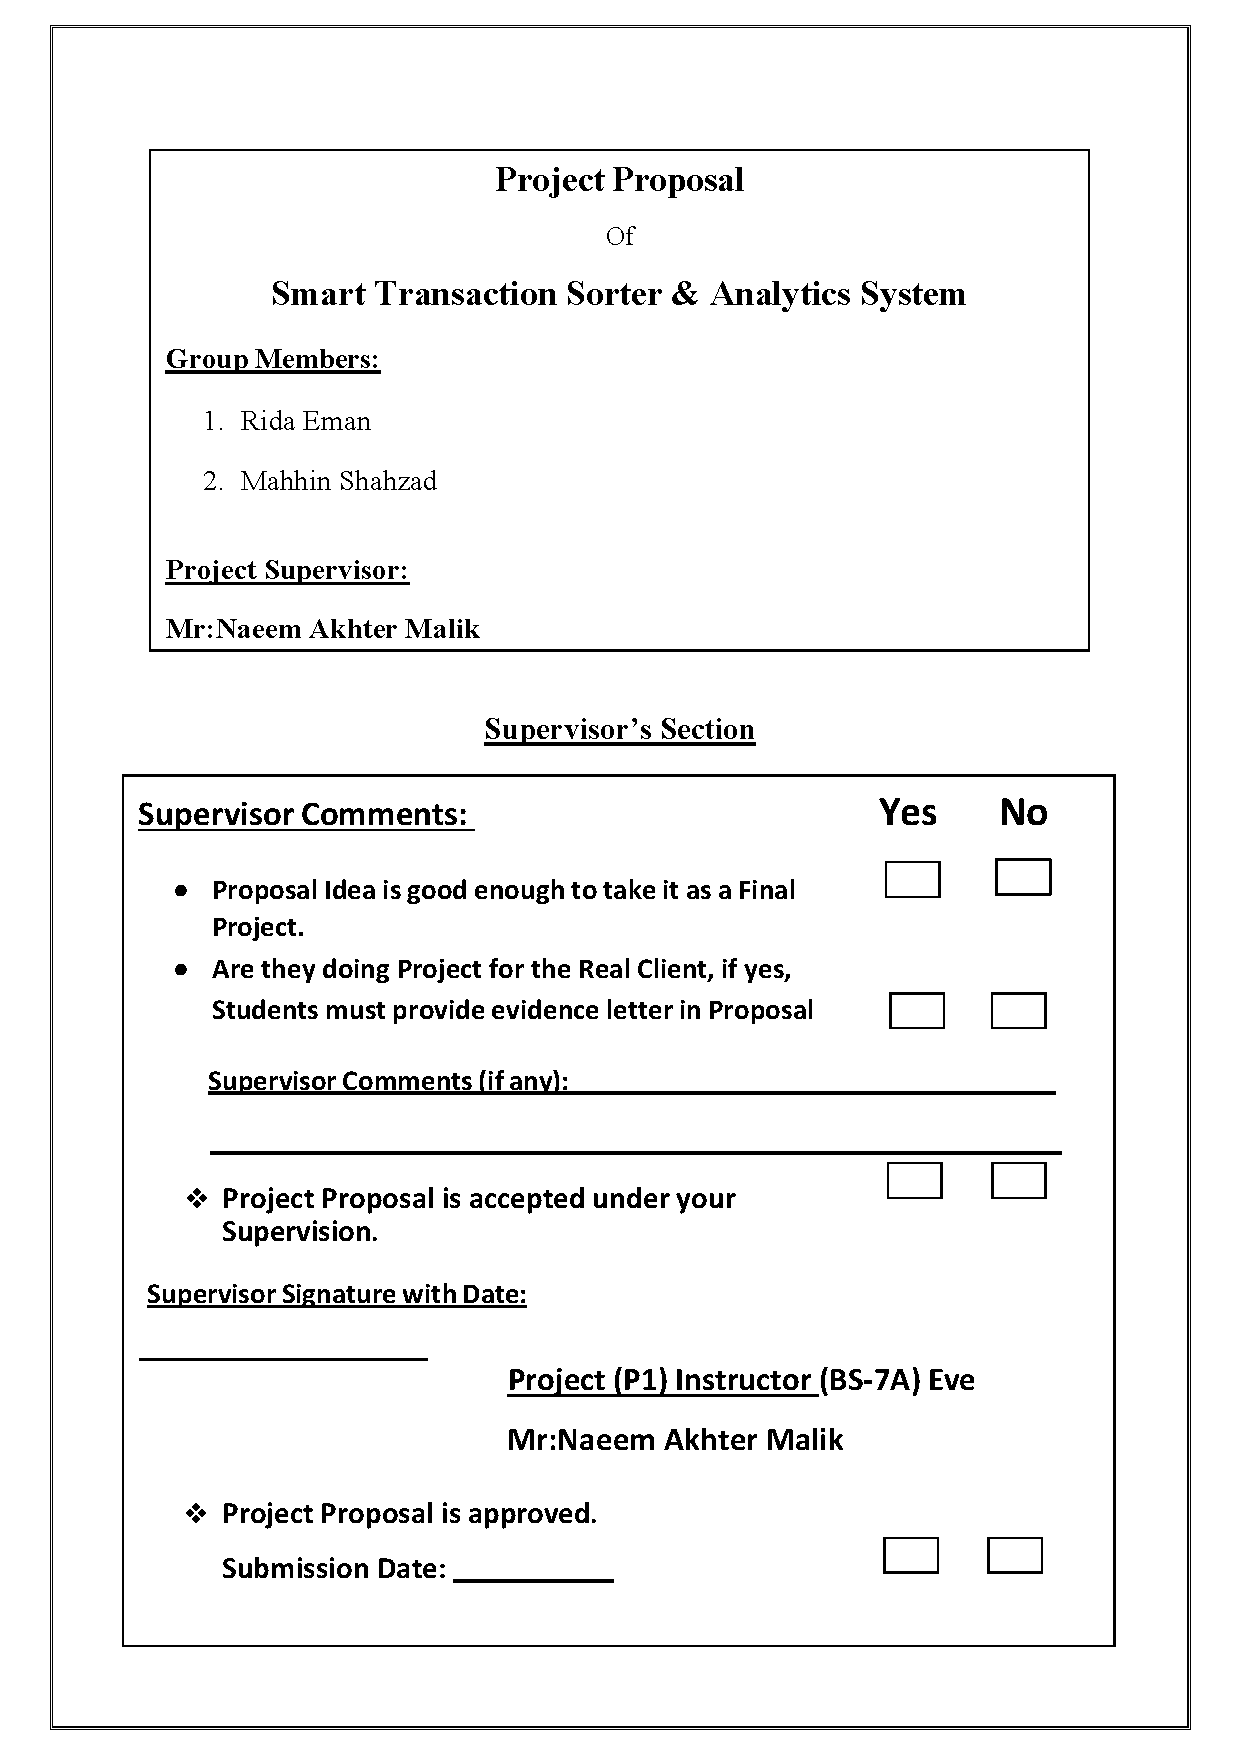
\includepdf[pages=-]{approval.pdf}
	
	% --- 3. Table of Contents ---
	\pagenumbering{roman} 
	\tableofcontents
	\newpage
	\listoffigures
	\newpage
	\listoftables
	\newpage
	\pagenumbering{arabic}

    % --- CHAPTERS ---
    
% =========================================================
% CHAPTER 1: INTRODUCTION
% =========================================================
\chapter{Introduction}

\section{Introduction}
The rise of the digital economy in Pakistan has been driven by the widespread adoption of fintech platforms such as Easypaisa, SadaPay, and JazzCash~\cite{baig2022future}. These services have empowered millions of users by simplifying payments and providing instant access to their complete transaction history. This readily available data holds the potential to offer valuable insights into personal spending habits. However, for most users, this potential remains untapped as the data is typically provided in raw formats (e.g., CSV files) without sophisticated analytical tools.

This report documents the Smart Transaction Sorter and Analytics system, a web-based application designed to unlock the value hidden within this raw financial data. The project's academic objective is to develop a functional, standalone tool that serves as a research-based feasibility study. The resulting application is structured as a practical blueprint for an intelligent analytics module. The long-term vision, while outside the immediate scope of this project, is that such a module could be pitched for integration into the very fintech platforms it complements, thereby closing the significant analytical gap in the current market.

\section{Problem Statement}
The problem is the absence of an integrated Business Intelligence (BI) and analytics layer in Pakistan digital wallets, prompting many users to request spending breakdown features online~\cite{reddit2023sadapay}. People export their data, move it into another tool, and tag each transaction by hand. It is a manual and time-consuming process.

\section{Proposed System}
The proposed system is a standalone, web-based application focused on delivering a complete workflow from raw CSV data to a finalized BI dashboard. To automate data preparation for the dashboard, an intelligent sorting component using Gemini API is included. The system aims to demonstrate feasibility using realistic transaction data while remaining independent from direct banking or wallet API integrations. The core functionality is broken down as follows:

\begin{enumerate}
	\item \textbf{Custom Category Management:} The user will first define their own set of personal spending categories (e.g., Groceries, Transport, Health \& Fitness).
	\item \textbf{CSV Data Ingestion:} The user then uploads their transaction history as a standard CSV file. This serves as the primary data input mechanism.
	\item \textbf{Intelligent Sorting Component:} A smart classification component, utilizing Gemini API, processes the raw data. It analyzes transaction descriptions and human-like notes/comments, mapping each entry to the most relevant category from the user's own custom list. This automated step moves beyond simple rule-based mapping to understand context, preparing the data accurately for the BI layer.
	\item \textbf{Interactive BI Visualization:} Once sorted, the data is presented to the user through an interactive Business Intelligence (BI) dashboard. This dashboard is the primary output and uses Metabase~\cite{metabase2024bi} to visualize spending breakdowns tailored to the user's personal financial structure.
	\item \textbf{Validation with Public Data:} To demonstrate the effectiveness and real-world applicability of the sorting component, the system will be tested and validated using a relevant public dataset. This dataset will contain transaction-like entries with descriptions and comments, allowing for rigorous evaluation of the classification accuracy without relying on proprietary user data.
\end{enumerate}
By leveraging a sorting mechanism powered by Gemini API, adaptable to user categories and validated on realistic transaction data, the application delivers personalized and accurate insights through its core BI and visualization dashboard.

\section{Survey of the Related Applications}
To establish the necessity of this project, this survey analyzes two distinct application categories: the local digital wallets that create the data and the problem, and the global expense trackers that represent existing but flawed solutions.

\subsection{A. Market Survey — Local Digital Wallets (Direct Context)}
A review of the official documentation for Pakistan's leading digital wallets confirms that while they excel at payments, they generally lack a mature, integrated analytics tool.
\begin{itemize}
	\item \textbf{SadaPay, NayaPay, \& Easypaisa:} These platforms reliably provide users with the ability to download their account statements or view transaction histories, with some confirming CSV export availability~\cite{nayapay2023documents}. However, comparative reviews confirm that both SadaPay and NayaPay lack advanced in-app auto-categorization features~\cite{arshad2025sadapay}, and their feature sets do not include built-in BI or smart analytics layers. Indeed, product growth studies for Easypaisa have proposed introducing AI-powered expense tracking (such as Paisa Pulse) to incentivize premium subscriptions and solve this automated budgeting gap~\cite{nextleap2023easypaisa}.
	\item \textbf{JazzCash:} While also providing standard statements, JazzCash recently announced a Spending Tracker feature~\cite{jazzcash2023tracker}. Based on its public introduction, this appears to be a basic tracking tool for monitoring budgets. While a positive step, it is distinct from a full-scale BI layer and does not offer the intelligent, personalized categorization that is central to this proposal.
\end{itemize}
\textit{Implication.} The local market either offers no native analytics or, at best, provides basic tracking. This creates a clear analytics vacuum and validates the need for a separate application to provide the missing intelligence.

\subsection{B. Indirect Comparators — Global CSV-Import Tools}
Global platforms like YNAB and Mint demonstrate the feasibility of the CSV-import workflow but are poorly suited to the local context and fail to solve the core problem of personalization.
\begin{itemize}
	\item \textbf{High-Friction Workflow:} Tools like YNAB and Mint, while powerful, still require significant manual effort after a CSV import to clean up data and assign categories line-by-line. This does not solve the primary issue of laborious manual work.
	\item \textbf{Lack of Personalization and Intelligence:} These platforms are separate, often paid services that use rigid, generic categorization systems. They lack the intelligent sorting component needed to learn and adapt to a user's own custom financial categories, failing the key protein bar test case.
	\item \textbf{Misaligned Business Model:} Their primary model is direct bank API integration, which is not the standard in the Pakistani market. Their CSV import tools are a secondary feature, not the core product.
\end{itemize}
\textit{Implication.} The global tools prove the CSV-to-analytics model is viable but highlight a gap for a more intelligent, low-friction, and personalized solution tailored to the realities of the local market. This project is designed specifically to fill that gap.

\subsection{C. Comparative Analysis Framework}

\subsubsection{The Keyword Inflexibility Problem}
Traditional personal finance tracking software relies heavily on rigid string-matching routines. These rule-based parsers search for specific, exact keywords to match an entry to a category. While computationally fast, this framework fails when processing real-world transaction statements.

Local digital wallet statements frequently include irregular text strings, merchant branch codes, or variable transfer notes. A rule-based system looking for "KFC" will completely miss strings like "KFC-ISB-05" or "KFC Centaurus". This limitation forces users to constantly maintain complex mapping tables.

In addition to branch codes, transactions often append dynamic transaction numbers, payment dates, or terminal identifiers to the description field. These changing characters create unique strings for every purchase, even when the merchant is identical. Because a static keyword parser cannot match these variants, the system leaves many transactions uncategorized, requiring constant manual updates. Over time, the administrative overhead of adjusting rules makes these tracking tools too tedious for average users to maintain.

\subsubsection{Semantic Adaptation and Intent Recognition}
The Smart Transaction Sorter addresses this limitation by using natural language processing. Instead of treating text strings as exact keys, the system processes transaction descriptions as contextual data. It evaluates the vocabulary, merchant references, and user comments together.

The underlying language model recognizes the real-world semantic intent behind variations in text. This allows the system to map "Paid to INDRIVE ISLAMABAD" to a user-defined "Transport" category automatically. This semantic approach removes the need for constant manual rules, reducing setup effort for the end-user.

By looking at the complete text, the classifier captures contextual hints that rule-based systems ignore. For instance, payment descriptions containing words like transfer, sending, or receiving are evaluated alongside the payment type to determine the core intent of the transaction. This ensures that the system handles unusual or brand-new merchant names correctly without needing direct user intervention. It allows the classification system to adjust to new spending patterns automatically, making the initial setup much simpler.

\section{Modules \& Sub-modules}
The system architecture will be broken down into the following modules and sub-modules to ensure a clear separation of concerns and facilitate iterative development.

\subsection{User \& Category Management Module}
This module will handle all user-facing administrative tasks and personalization features.
\begin{itemize}
	\item \textbf{Authentication Submodule:} This submodule is responsible for secure user registration, login, logout, and session management to ensure data privacy.
	\item \textbf{Category CRUD Submodule:} This provides the interface and backend logic for users to Create, Read, Update, and Delete (CRUD) their personalized list of spending categories.
\end{itemize}

\subsection{Data Ingestion Module}
This module serves as the primary data entry point for transaction histories.
\begin{itemize}
	\item \textbf{File Upload Submodule:} This submodule provides the secure, user-facing web form for uploading transaction data in CSV format.
	\item \textbf{CSV Validation Submodule:} This is a backend service that parses the uploaded file and verifies its structural integrity, ensuring required columns (e.g., Date, Description, Amount) are present.
\end{itemize}

\subsection{Intelligent Sorting Module}
This module contains the core data processing and classification logic.
\begin{itemize}
	\item \textbf{Data Pre-processing Submodule:} This submodule cleans and standardizes the validated data, converting data types (e.g., string dates to date objects) to prepare it for classification.
	\item \textbf{Classification Engine Submodule:} This is the smart component that takes a transaction's text and the user's custom category list as input, and outputs the most probable category.
	\item \textbf{Database Persistence Submodule:} This submodule saves the processed transaction data, along with its newly assigned category, into the database.
\end{itemize}

\subsection{BI \& Visualization Module}
This module is responsible for presenting the final analytical output to the user.
\begin{itemize}
	\item \textbf{Token Authentication Submodule:} This is a backend service that compiles secure, signed JSON Web Tokens containing user session parameters using the HMAC-SHA256 algorithm.
	\item \textbf{Dashboard Rendering Submodule:} This is the frontend component that renders the securely embedded Metabase dashboard inside an iframe, applying the token parameters to display user-scoped charts and statistics.
\end{itemize}

\section{Primary Actors}
The system is designed for a single primary actor:
\begin{itemize}
	\item \textbf{The User:} An individual who wants to analyze their personal financial transaction history. The User will be able to perform the following actions:
	\begin{itemize}
		\item Register for an account and log in securely.
		\item Create and manage their own personalized list of spending categories.
		\item Upload their transaction history in CSV format.
		\item View the interactive BI dashboard with visualizations of their spending.
		\item (Optional) Review and manually correct any automated classifications.
	\end{itemize}
\end{itemize}

\section{Tools \& Techniques}
The project uses a modern, stable technology stack to ensure scalability and maintainability.
\begin{itemize}
	\item \textbf{Backend Framework:} Python with the Django Framework is used to build the server-side logic, manage URLs, and handle database interactions.
	\item \textbf{Database:} PostgreSQL is the confirmed database target for the final system because it supports reliable relational storage, indexing, and production deployment.
	\item \textbf{Data Processing:} Python CSV handling, Django forms, and model validation are used for efficient parsing, validation, and storage of uploaded transaction data.
	\item \textbf{Intelligent Sorting:} Gemini API is used to implement the classification component through structured prompts, JSON responses, confidence scoring, and category validation.
	\item \textbf{Frontend Visualization:} Metabase is used as the Business Intelligence layer and is embedded into the Django interface through a secure dashboard URL.
	\item \textbf{Web Technologies:} The user interface is built with Django templates, HTML, CSS, JavaScript, Bootstrap, and Jazzmin for the administrative interface.
\end{itemize}

\section{Process Model \& Design Approach}
The project will be developed using an Iterative and Incremental process model. This approach is well-suited for a modular system, as it allows for the development and testing of each component in successive cycles or iterations.

The development will proceed by building and testing each module individually before integrating them into a cohesive whole. This allows for early feedback, easier debugging, and a more manageable workflow. The design approach will follow the Model-View-Template (MVT) architectural pattern, which is native to the Django framework and provides a clear separation between data logic, business logic, and user interface.

\section{Project Plan}
The project timeline is scheduled over approximately seven months (30 weeks), visualized in the Gantt chart in Figure \ref{fig:gantt} below. The plan prioritizes documentation and core feature development first, followed by the integration of the intelligent sorting component and finalization.

\begin{figure}[H]
	\centering
	\resizebox{\textwidth}{!}{
		\begin{ganttchart}[
			vgrid,
			hgrid,
			bar/.append style={fill=blue!50},
			milestone/.append style={fill=red!70}
			]{1}{30}
			\gantttitle{Project Timeline (Weeks)}{30} \\
			\gantttitlelist{1,...,30}{1} \\
			
			% Phase 1: Documentation & Initial Setup
			\ganttgroup{Phase 1: Planning \& Design}{1}{8} \\
			\ganttmilestone[name=p1]{Proposal Submission}{1} \ganttnewline
			\ganttlinkedbar[name=srs]{SRS Documentation}{2}{3} \ganttnewline
			\ganttlinkedbar[name=uc]{Use Case Diagrams}{3}{5} \ganttnewline
			\ganttlinkedbar[name=ui]{Initial UI/UX Design}{5}{8} \ganttnewline
			
			% Phase 2: Core CSV & BI Development
			\ganttgroup{Phase 2: Core Feature Development}{9}{18} \\
			\ganttlinkedbar[name=data]{Develop Data Ingestion (CSV)}{9}{12} \ganttnewline
			\ganttlinkedbar[name=db]{Database \& Backend Setup}{11}{14} \ganttnewline
			\ganttlinkedbar[name=bi]{Develop BI \& Visualization Module}{13}{18} \ganttnewline
			
			% Phase 3: AI Integration & Testing
			\ganttgroup{Phase 3: AI Integration}{19}{25} \\
			\ganttlinkedbar[name=ai]{Develop Intelligent Sorting Module}{19}{22} \ganttnewline
			\ganttlinkedbar[name=integ]{Integrate Sorting with Main App}{23}{25} \ganttnewline
			
			% Phase 4: Finalization & Reporting
			\ganttgroup{Phase 4: Finalization \& Reporting}{26}{30} \\
			\ganttlinkedbar[name=test]{End-to-End Testing \& Bug Fixing}{26}{28} \ganttnewline
			\ganttlinkedbar[name=doc]{Final Report Documentation}{28}{29} \ganttnewline
			\ganttmilestone[name=p2]{Final Presentation}{30}
			
			% Links
			\ganttlink{p1}{srs}
			\ganttlink{srs}{uc}
			\ganttlink{uc}{ui}
			\ganttlink{ui}{data}
			\ganttlink{data}{db}
			\ganttlink{db}{bi}
			\ganttlink{bi}{ai}
			\ganttlink{ai}{integ}
			\ganttlink{integ}{test}
			\ganttlink{test}{doc}
			\ganttlink{doc}{p2}
		\end{ganttchart}
	}
	\caption{Project development timeline presented as a Gantt chart.}
	\label{fig:gantt}
\end{figure}

\section{Socio-Economic Context of FinTech in Pakistan}

\subsection{The Shift to Mobile Banking Ecosystems}
The financial landscape in Pakistan has changed rapidly due to the growth of branchless banking platforms. Services like Easypaisa, JazzCash, NayaPay, and SadaPay have enabled millions of individuals to manage money digitally. This has led to a massive increase in transaction volumes across a variety of user demographics.

Despite this growth in digital transactions, financial literacy tools have not kept pace. Most wallet providers optimize their interfaces for quick payments rather than long-term asset management. Users are left with unstructured text logs that do not offer clear visibility into their personal cash flows.

The absence of native tracking features makes it hard for users to build positive saving habits. Digital statements show when and where money was spent, but they don't help users understand their spending patterns. This gap in service creates a clear need for secondary analytical tools that can organize cash flows.

\subsection{The Cognitive Load of Unstructured Financial Data}
Raw data statements exported as CSV files create an analytical barrier for everyday consumers. Disorganized rows of dates and numeric strings make manual categorization tedious and frustrating. This data complexity often prevents users from maintaining consistent personal budgets.

The lack of a domestic personal finance management standard highlights the need for an automated layer. A standalone utility that cleans irregular formats and presents data visually makes financial tracking accessible. This system provides a practical blueprint for improving consumer financial awareness in the local market.

By automating the sorting task, the system removes the mental effort required to manage personal accounts. Users no longer need to spend hours grouping transactions by hand or deciphering vague merchant text. This convenience encourages regular budget reviews, helping individuals make better financial decisions.

\subsection{Empirical Challenges in Local Financial Text Processing}
The development of automated financial tracking utilities within the Pakistani fintech ecosystem faces significant text-processing challenges. Unlike international banking data, which often adheres to standardized merchant category codes and clean identification logs, local transaction logs from mobile wallets and domestic bank statements are notoriously unpredictable. These records frequently combine multiple languages, structural variations, and random numbers within a single description string.

The core text processing issues can be broken down into three distinct semantic categories:
\begin{itemize}
    \item \textbf{Alphanumeric Fragmentation and Dynamic IDs}: Local statements regularly interweave merchant identifiers with variable transactional sequences. For example, a single merchant transaction might append unique billing serials, date numbers, or terminal codes directly to the shop name. Because these codes change with every single purchase, traditional string-matching utilities fail completely. The text parser cannot determine where the stable merchant identifier ends and where the dynamic transaction counter begins, creating severe classification friction.
    \item \textbf{Bilingual Inconsistencies and Romanized Script}: Financial text logs in the local market rely heavily on Romanized Urdu phrasing mixed with standard English financial terms. Transaction notes routinely feature terms like bhai, shukriya, khana, or udhaar right alongside terms like funds transfer or bill payment. Furthermore, phonetic variations introduce massive structural differences. The same target concept or location can be spelled in multiple ways across different applications, requiring an analytics system that can recognize underlying semantic intent rather than relying on strict spelling matches.
    \item \textbf{Cryptic Merchant Abbreviations}: Point of sale machines and digital payment portals frequently truncate merchant listings into short, compressed character chains to fit narrow statement interfaces. A clear storefront name is often reduced to a confusing set of initials combined with local city or branch indicators. Without an intelligent natural language processing layer that evaluates the complete contextual signature of the text string, basic keyword rules treat these shortened tags as completely separate entities, leaving them entirely uncategorized.
\end{itemize}

    
% =========================================================
% CHAPTER 2: REQUIREMENTS SPECIFICATION
% =========================================================
\chapter{Requirements Analysis}

\section{Purpose}
The purpose of the Smart Transaction Sorter and Analytics System is to provide users with an intelligent, automated way to analyze their personal financial spending. This web application uses Artificial Intelligence (AI) to categorize raw transaction data (from CSV files) and instantly convert it into clear, visual charts, eliminating the need for hours of frustrating manual work.

\section{Project Scope}
The scope of this project is a standalone, web-based tool that accepts a financial history file (CSV), uses AI to categorize every line based on user-defined labels, and presents the results on a BI Dashboard. The system includes User authentication, Category Management, CSV Upload/Validation, AI Sorting Logic, Data Persistence, and a Visualization Dashboard.

\begin{itemize}
	\item \textbf{In Scope:} User login, Category creation, CSV parsing, AI classification, Dashboard charts.
	\item \textbf{Out of Scope:} Direct integration (API) with bank/wallet accounts, payment processing, or real-time transaction tracking.
\end{itemize}

\section{Definitions, Acronyms, and Abbreviations}
\renewcommand{\arraystretch}{1.5}
\begin{longtable}{|p{4cm}|p{10.5cm}|}
	\hline
	\textbf{Term/Abbreviation} & \textbf{Definition} \\
	\hline
	\endfirsthead
	\hline
	\textbf{Term/Abbreviation} & \textbf{Definition} \\
	\hline
	\endhead
	STS & Smart Transaction Sorter (The name of this application). \\ \hline
	AI & Artificial Intelligence (The component that performs automatic classification). \\ \hline
	CSV & Comma-Separated Values (The standard file format for data input/upload). \\ \hline
	BI & Business Intelligence (Refers to the analytical dashboard and visualization tools). \\ \hline
	DB & Database (The system storage where user and financial data are saved). \\ \hline
\end{longtable}

\section{Document Overview}
This document describes the requirements for the Smart Transaction Sorter and Analytics System (STS). It serves as the single reference point for what the system must do and how well it must perform. The STS acts as a complimentary Business Intelligence layer for existing digital wallets and bank applications that currently only offer raw data exports.

\section{Functional Requirements}

\subsection{Security Management}

\subsubsection{Process Sign Up}
\begin{longtable}{|p{2.5cm}|p{12cm}|}
	\hline
	\textbf{ID} & \textbf{Requirement Description} \\
	\hline
	SRS-1 & The system shall allow new users to securely register by providing a username, email, and password. \\ \hline
	SRS-2 & The system must validate that the email address is unique and not already registered. \\ \hline
	SRS-3 & The system shall store user passwords using a strong one-way hash (never in plain text). \\ \hline
	SRS-4 & Upon successful registration, the system shall create a dedicated, isolated database scope for the user. \\ \hline
\end{longtable}

\subsubsection{Process Sign In / Logout}
\begin{longtable}{|p{2.5cm}|p{12cm}|}
	\hline
	\textbf{ID} & \textbf{Requirement Description} \\
	\hline
	SRS-5 & The system shall allow registered users to log in securely using their credentials. \\ \hline
	SRS-6 & The system shall use HTTPS/SSL for all data transfer between the client and server to prevent interception. \\ \hline
	SRS-7 & The system shall allow users to securely log out, terminating their current session. \\ \hline
\end{longtable}

\subsection{Category Management}

\subsubsection{Create Spending Category}
\begin{longtable}{|p{2.5cm}|p{12cm}|}
	\hline
	\textbf{ID} & \textbf{Requirement Description} \\
	\hline
	SRS-8 & The system shall allow users to create new, personalized spending category labels (e.g., "Groceries", "Utilities"). \\ \hline
	SRS-9 & The system shall validate that the category name is not a duplicate within the user's profile. \\ \hline
	SRS-10 & The system shall ensure all created categories are immediately available for the AI Sorting Engine to use. \\ \hline
\end{longtable}

\subsubsection{Manage Spending Categories}
\begin{longtable}{|p{2.5cm}|p{12cm}|}
	\hline
	\textbf{ID} & \textbf{Requirement Description} \\
	\hline
	SRS-11 & The system shall allow users to view a list of all their existing categories. \\ \hline
	SRS-12 & The system shall allow users to edit the name of an existing category. \\ \hline
	SRS-13 & The system shall allow users to delete a category (and optionally reassign its associated transactions). \\ \hline
\end{longtable}

\subsection{Data Ingestion Management}

\subsubsection{Upload Transaction File (CSV)}
\begin{longtable}{|p{2.5cm}|p{12cm}|}
	\hline
	\textbf{ID} & \textbf{Requirement Description} \\
	\hline
	SRS-14 & The system shall provide a simple interface for the user to upload a transaction history file. \\ \hline
	SRS-15 & The system is constrained to accepting only CSV (Comma-Separated Values) file formats. \\ \hline
	SRS-16 & The system shall provide a progress indicator or status feedback during the upload process. \\ \hline
\end{longtable}

\subsubsection{File Validation}
\begin{longtable}{|p{2.5cm}|p{12cm}|}
	\hline
	\textbf{ID} & \textbf{Requirement Description} \\
	\hline
	SRS-17 & The system shall check the uploaded file for necessary columns (specifically: Date, Description, and Amount). \\ \hline
	SRS-18 & The system shall provide clear, user-friendly error messages if the file structure is invalid or missing data. \\ \hline
	SRS-19 & The system shall reject files that exceed a predefined size limit to maintain performance. \\ \hline
\end{longtable}

\subsection{Intelligent Sorting Management}

\subsubsection{Process Transactions (AI Sorting)}
\begin{longtable}{|p{2.5cm}|p{12cm}|}
	\hline
	\textbf{ID} & \textbf{Requirement Description} \\
	\hline
	SRS-20 & The system shall use a smart classification model (AI) to read transaction descriptions from the uploaded file. \\ \hline
	SRS-21 & The system shall automatically assign the most relevant custom category to each transaction. \\ \hline
	SRS-22 & The system shall utilize Gemini API for the classification logic. \\ \hline
\end{longtable}

\subsubsection{Data Persistence \& Saving}
\begin{longtable}{|p{2.5cm}|p{12cm}|}
	\hline
	\textbf{ID} & \textbf{Requirement Description} \\
	\hline
	SRS-23 & The system shall securely save the processed transaction data, including the new category label, to the user's database. \\ \hline
	SRS-24 & The system shall ensure that once categorized, the financial history persists until explicitly deleted by the user. \\ \hline
\end{longtable}

\subsection{Analytics Management}

\subsubsection{View Dashboard}
\begin{longtable}{|p{2.5cm}|p{12cm}|}
	\hline
	\textbf{ID} & \textbf{Requirement Description} \\
	\hline
	SRS-25 & The system shall display a primary BI (Business Intelligence) dashboard view after processing is complete. \\ \hline
	SRS-26 & The dashboard shall be interactive, allowing users to hover over elements for more details. \\ \hline
\end{longtable}

\subsubsection{View Spending Breakdown}
\begin{longtable}{|p{2.5cm}|p{12cm}|}
	\hline
	\textbf{ID} & \textbf{Requirement Description} \\
	\hline
	SRS-27 & The system shall display clear charts (e.g., pie charts) visualizing total spending broken down by custom categories. \\ \hline
	SRS-28 & The system shall calculate and display total expenditure for the uploaded period. \\ \hline
\end{longtable}

\subsection{Administrator Management}

\subsubsection{Admin Panel Access}
\begin{longtable}{|p{2.5cm}|p{12cm}|}
	\hline
	\textbf{ID} & \textbf{Requirement Description} \\
	\hline
	SRS-29 & The System Administrator must use distinct credentials to log in to the dedicated administrative interface. \\ \hline
	SRS-30 & The Admin Panel shall be secured and inaccessible to standard users. \\ \hline
\end{longtable}

\subsubsection{User Account Management}
\begin{longtable}{|p{2.5cm}|p{12cm}|}
	\hline
	\textbf{ID} & \textbf{Requirement Description} \\
	\hline
	SRS-31 & The Admin shall have the ability to View and Search for any registered user account. \\ \hline
	SRS-32 & The Admin shall have the ability to Create, Edit, or Delete user accounts if necessary. \\ \hline
	SRS-33 & The Admin shall have read-only access to view user-created Categories and processed Transactions for auditing purposes. \\ \hline
\end{longtable}

\section{Non-Functional Requirements}

\subsection{Security}
\begin{itemize}
	\item \textbf{Account Protection:} User passwords must be stored using a strong one-way hash.
	\item \textbf{Session Security:} The system must use HTTPS for all communication to prevent data interception.
	\item \textbf{User Isolation:} A user's data must be completely isolated and inaccessible to any other user.
\end{itemize}

\subsection{Usability}
\begin{itemize}
	\item The interface must be intuitive, clean, and fully mobile-responsive.
	\item Training time for a normal user to understand the upload and sort process should be minimal (intuitive design).
\end{itemize}

\subsection{Reliability}
\begin{itemize}
	\item The system must be available and function correctly 99.5\% of the time.
	\item In any error scenario, the system must provide an appropriate message and retain the state of the user's data (no silent failures).
\end{itemize}

\subsection{Performance}
\begin{itemize}
	\item \textbf{File Processing Time:} A standard file (up to 500 transactions) must be processed, sorted by the AI, and ready for viewing within 60 seconds.
	\item The system dashboard should load visualization results in under 3 seconds after processing is complete.
\end{itemize}

\subsection{Design Constraints}
\begin{itemize}
	\item \textbf{Technology Stack:} Must use Python (Django Framework) for the backend logic.
	\item \textbf{Database:} Designed for use with PostgreSQL for scalability.
	\item \textbf{AI Service:} The system must utilize Gemini API for intelligent transaction classification.
	\item \textbf{Architecture:} The code must follow the MVT (Model-View-Template) architectural pattern.
\end{itemize}

\subsection{Data Ownership \& Business Rules}
\begin{itemize}
	\item \textbf{Data Ownership:} All uploaded data remains the intellectual property of the User.
	\item \textbf{No Third-Party Sharing:} User financial data may not be shared, sold, or exposed to any third party.
	\item \textbf{Persistence:} Processed data remains available until the user explicitly decides to delete it.
\end{itemize}

\section{External Interface Requirements}

\subsection{User Interfaces}
The user interface will be entirely web-based, optimized for responsive viewing on desktop and mobile devices. Key interfaces include:
\begin{itemize}
	\item Login/Registration Forms.
	\item Custom Category Management Form (CRUD interface).
	\item CSV File Upload Interface with progress/status feedback.
	\item Interactive BI Dashboard embedded through Metabase.
	\item A secure Admin Panel (for System Administrator use only).
\end{itemize}

\subsection{Hardware Interfaces}
No specialized hardware is required. The system will interface with standard internet-supported client devices (PC, laptop, mobile, tablet).

\subsection{Software Interfaces}
The system interfaces with the following software components:
\begin{itemize}
	\item \textbf{Python / Django:} Primary backend web application and API interface.
	\item \textbf{PostgreSQL:} Database management system for data persistence.
	\item \textbf{Python CSV and Django Forms:} Used for data parsing, validation, and persistence into database models.
	\item \textbf{Gemini API:} The core AI service used for transaction classification.
	\item \textbf{Metabase:} Business Intelligence tool used for dashboard visualization and embedded analytics.
\end{itemize}

\section{Detailed Functional Requirement Scenarios and Edge Cases}
To ensure the system remains stable under varied real-world usage, the core functional requirements must be evaluated against realistic data flows, alternative execution paths, and exception boundaries. This section outlines the sequential operations, alternative states, and failure recovery protocols for the four primary processing hubs of the application.

\subsection{Sign Up and Authentication Scenarios}
The user onboarding process represents the initial security gate of the application. To protect personal financial data, registration and authentication must enforce strict boundaries at the database and application levels.
\subsubsection{Sequential Processing Logic}
The registration sequence is initiated when a visitor requests the signup form. The Django backend generates a unique Cross-Site Request Forgery (CSRF) token, binds it to the session, and renders the form fields. The user must provide a username, a unique email address, a password, and a password confirmation. Upon submission, the backend performs form-level checks:
\begin{enumerate}
	\item \textbf{Syntax Verification:} The email address is checked against a standard format regex pattern to confirm structural validity.
	\item \textbf{Duplicate Auditing:} The database is queried to ensure the email address does not match any existing record.
	\item \textbf{Complexity Evaluation:} The password string is audited against complexity rules, verifying it contains at least eight characters, including numerical and alphabetical values.
	\item \textbf{Password Matching:} The password and confirmation strings are checked for character-for-character equality.
\end{enumerate}
If all validations pass, the Django authentication module hashes the password string using the PBKDF2 algorithm with a SHA-256 hash. The system opens a database transaction, saves the user record, generates a personalized default category set (e.g., Utilities, Groceries, Transport), commits the transaction, and redirects the user to the login screen.

\subsubsection{Alternate Courses and Exception Handling}
During registration, input errors or system faults can redirect the execution flow:
\begin{itemize}
	\item \textbf{Duplicate Account Conflict (Alternate Course):} If the database query identifies an existing user account registered under the submitted email, the system halts the creation process. The backend raises a form validation error, re-renders the registration page, and displays a notice stating that the email address is already in use.
	\item \textbf{Password Complexity Failure (Alternate Course):} If the password contains fewer than eight characters or fails complexity rules, the validation script blocks database entry. The system flags the password field and displays a message explaining the length and character requirements.
	\item \textbf{Database Transaction Timeout (Exception Path):} In the event of high database lock contention or server latency, the registration write operation may time out. The application catches the database transaction error, rolls back any partial database updates, logs the system error, and redirects the user to a page explaining that the server is temporarily busy, prompting them to try again.
\end{itemize}

\subsection{CSV Ingestion and Parsing Scenarios}
The ingestion pipeline converts external financial statement files into internal database records. Since banks and wallet services generate statement CSVs with different layouts, the ingestion service must handle files with structural variations.
\subsubsection{Sequential Processing Logic}
When an authenticated user requests a file upload, the application validates the file extension, selection of ingestion pathway, and size before opening the data stream. The ingestion pipeline supports uploading multiple CSV files simultaneously. If the files pass the initial boundaries, the Pandas library is initialized to read the CSV content of each file. The sequence executes as follows:
\begin{enumerate}
	\item \textbf{File Stream Buffering:} The uploaded files are read into memory as byte streams, avoiding disk-write latency.
	\item \textbf{Pathway Routing and Header Extraction:} The system routes each file stream based on the selected import pathway (Generic CSV Template or NayaPay Mobile Statement). For standard files, the parser matches columns against expected fields (Date, Description, and Amount) using case-insensitive mapping and predefined aliases. For NayaPay statements, the parser automatically maps specialized wallet export fields.
	\item \textbf{Data Cleaning:} The system loops through each row in the dataframe. It trims trailing spaces from descriptions, extracts transaction references, and removes currency symbols (such as Rs. or PKR) and thousands-separator commas from the amount values.
	\item \textbf{Transaction Batching:} The cleaned records are converted into transaction model instances and appended to a list for bulk database insertion.
\end{enumerate}
Once the batch list is fully populated, the Django ORM executes a single bulk insert operation to save the transactions.

\subsubsection{Alternate Courses and Exception Handling}
Data parsing must account for incomplete files, irregular cell contents, and format mismatches:
\begin{itemize}
	\item \textbf{Missing Column Headers (Alternate Course):} If the header row lacks one of the required columns (Date, Description, or Amount) and no alias matches are found, the Pandas parser halts. The system aborts the upload, discards the buffered stream, and renders a message stating which mandatory column is missing.
	\item \textbf{Non-Numeric Amount Formatting (Alternate Course):} When a row contains non-numeric text in the Amount column (such as ``N/A'' or ``FREE''), the numeric coercion module converts the entry to a null value. The row filter detects this null value and skips the row, recording it in the import log while continuing to process the other rows.
	\item \textbf{Encoding Mismatch Exception (Exception Path):} Financial statements may be encoded in UTF-8 or legacy formats like ISO-8859-1. If the parser encounters characters it cannot read, a decoding exception is raised. The application catches the exception, closes the stream, and displays a message asking the user to save the CSV in standard UTF-8 format.
\end{itemize}

\subsection{AI Classification and Inference Scenarios}
The Gemini API classification engine automates the assignment of spending categories using semantic natural language processing.
\subsubsection{Sequential Processing Logic}
When the user triggers the AI sorting function, the backend verifies that the user has custom categories and that there are uncategorized transactions. The classification sequence proceeds as follows:
\begin{enumerate}
	\item \textbf{Taxonomy Loading:} The system fetches the list of custom categories defined by the user.
	\item \textbf{Transaction Batching:} Uncategorized transactions are divided into batches of 25 to balance API payload size and network response latency.
	\item \textbf{Prompt Construction:} The engine compiles a structured prompt containing the candidate labels and the batch of transactions.
	\item \textbf{Gemini Classification:} The text descriptions are evaluated against the user's category list. The Gemini model calculates a confidence score for each category.
	\item \textbf{Confidence Assessment:} The engine checks the highest confidence score against the 0.5 safety threshold. If it exceeds the threshold, the category is assigned.
\end{enumerate}
The database is then updated with the category assignments.

\subsubsection{Alternate Courses and Exception Handling}
The AI sorting pipeline must handle low-confidence results and service interruptions:
\begin{itemize}
	\item \textbf{Low-Confidence Bypass (Alternate Course):} If the highest confidence score for a transaction falls below 0.5, the engine flags the prediction as uncertain. The system assigns the default label ``Uncategorized'' and stores the model's top guess as a suggestion, allowing the user to review the record later.
	\item \textbf{Empty Taxonomy Interception (Alternate Course):} If a user runs the classification engine without defining any categories, the application bypasses model execution. It marks all pending rows as ``Uncategorized'' and notifies the user to configure custom categories.
	\item \textbf{API Request Timeout (Exception Path):} High network latency or API rate limits may cause classification requests to time out. The application is configured to retry the request once. If the retry fails, the engine halts, rolls back the batch update, and displays a warning to the user, ensuring that no partially sorted records are left in the database.
\end{itemize}

\subsection{Dashboard Aggregation and Visualization Scenarios}
The analytics module provides secure data visualization dashboards using embedded Metabase resources.
\subsubsection{Sequential Processing Logic}
When a user accesses the dashboard, the application generates a secure, token-authorized iframe. The sequence runs as follows:
\begin{enumerate}
	\item \textbf{Configuration Audit:} The system checks the environment configuration settings to retrieve the Metabase site URL and embedding secret key.
	\item \textbf{Token Signature:} The backend compiles a JSON Web Token signed with the HMAC-SHA256 algorithm. The token contains the active user's identification number as a query filter parameter.
	\item \textbf{URL Construction:} The system appends the signed token to the Metabase dashboard site path, creating a secure embedding URL.
	\item \textbf{Frontend Embedding:} The Django template receives the URL and renders the Metabase dashboard inside an iframe within a glassmorphic dashboard container. The Metabase server filters the database queries dynamically using the user ID parameter.
\end{enumerate}

\subsection{Alternate Courses and Exception Handling}
The dashboard aggregation system must handle empty datasets and authorization issues:
\begin{itemize}
	\item \textbf{Missing Key Interception (Alternate Course):} If the Metabase secret key is missing from environment configurations, the dashboard view intercepts the error. It blocks the iframe generation and renders a warning banner explaining how to configure the environment settings.
	\item \textbf{Expired Session Token (Alternate Course):} The JSON Web Token contains an expiration timestamp set to 10 minutes. If the user keeps the dashboard open past this limit, Metabase displays a signature expired error. Refreshing the dashboard page generates a fresh token, restoring the view.
	\item \textbf{Zero Record State (Exception Path):} If the user has no transactions, the database queries return empty sets. Metabase displays empty visual states on the dashboard, explaining that data needs to be uploaded to populate the charts.
\end{itemize}

    
% =========================================================
% CHAPTER 3: USE CASE ANALYSIS
% =========================================================
\chapter{Use Case Analysis}


\section{Use Case Diagram}
The Use Case Diagram provides a high-level overview of the system's interactions with the primary actors (User and System Administrator).

\begin{figure}[H]
	\centering
	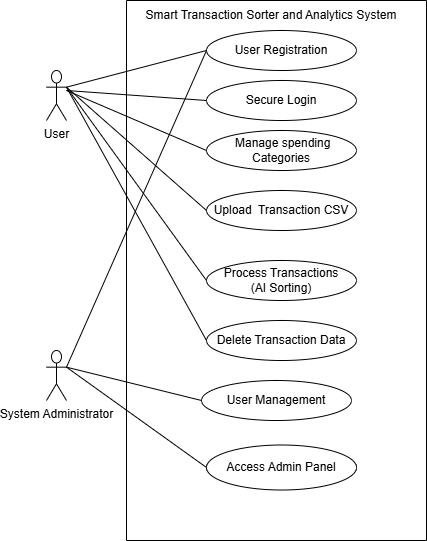
\includegraphics[width=0.9\textwidth, height=13cm, keepaspectratio]{usecase_diagram.png}
	\caption{Smart Transaction Sorter System Use Case Diagram}
	\label{fig:usecase_diagram}
\end{figure}

\section{Fully Dressed Use Case Scenarios}

\subsection{User Access \& Authentication}

% --- USE CASE 1.1 ---
\subsubsection{Use Case 1.1: User Registration}
\begin{tabularx}{\textwidth}{|L|R|}
	\hline
	Use Case ID & 1.1 \\ \hline
	Use Case Name & User Registration \\ \hline
	Actor & User \\ \hline
	Description & A new user creates a secure account to access the system features. \\ \hline
	Preconditions & User has a valid email address and internet access. \\ \hline
	Postconditions & A new user account is created in the database, and the user is redirected to the login page. \\ \hline
	Priority & High \\ \hline
	Normal Course & 
	\begin{normalsteps}
		\item User navigates to the application landing page.
		\item User selects "Register".
		\item System displays the registration form.
		\item User enters Name, Email, and Password (twice).
		\item System validates the input format.
		\item System hashes the password and saves the new user record.
		\item System displays a success message.
	\end{normalsteps} \\ \hline
	Alternative Courses & 
	\textbf{5a. Weak Password:} 
	\begin{altsteps}
		\item System detects password does not meet security complexity requirements.
		\item System prompts user to choose a stronger password.
	\end{altsteps} 
	\textbf{6a. Email Already Exists:} 
	\begin{altsteps}
		\item Database check confirms the email is already registered.
		\item System displays error: "Account already exists".
		\item System prompts user for Login.
	\end{altsteps} \\ \hline
	Exceptions & Database connection failure prevents account creation. \\ \hline
	Special Req. & Passwords must be hashed using a strong algorithm (e.g., PBKDF2 or Argon2) before storage. \\ \hline
\end{tabularx}

\newpage

% --- USE CASE 1.2 ---
\subsubsection{Use Case 1.2: Secure Login}
\begin{tabularx}{\textwidth}{|L|R|}
	\hline
	Use Case ID & 1.2 \\ \hline
	Use Case Name & Secure Login \\ \hline
	Actor & User, System Administrator \\ \hline
	Description & Users or Admins log in to access their respective dashboards. \\ \hline
	Preconditions & User/Admin must have a registered account. \\ \hline
	Postconditions & Actor is authenticated, a session is established, and they are redirected to their authorized dashboard. \\ \hline
	Priority & High \\ \hline
	Normal Course & 
	\begin{normalsteps}
		\item Actor navigates to the Login page.
		\item Actor enters Email and Password.
		\item System verifies credentials against the database.
		\item System generates a secure session token.
		\item System identifies the role (User or Admin) and redirects to the appropriate Dashboard.
	\end{normalsteps} \\ \hline
	Alternative Courses & 
	\textbf{3a. Invalid Credentials:} 
	\begin{altsteps}
		\item System detects email/password do not match.
		\item System displays "Invalid Login" error.
		\item System allows retry (limit 5 attempts).
	\end{altsteps} \\ \hline
	Exceptions & Account is locked due to too many failed attempts. \\ \hline
	Special Req. & Communication must occur over HTTPS. \\ \hline
\end{tabularx}

\newpage

\subsection{Core Configuration}

% --- USE CASE 2.1 ---
\subsubsection{Use Case 2.1: Manage Spending Categories}
\begin{tabularx}{\textwidth}{|L|R|}
	\hline
	Use Case ID & 2.1 \\ \hline
	Use Case Name & Manage Spending Categories \\ \hline
	Actor & User \\ \hline
	Description & User defines the custom labels (e.g., "Gym", "Groceries") that the AI will use for sorting. \\ \hline
	Preconditions & User is logged in. \\ \hline
	Postconditions & The list of categories is updated in the database and ready for the AI engine. \\ \hline
	Priority & High \\ \hline
	Normal Course & 
	\begin{normalsteps}
		\item User navigates to "Manage Categories".
		\item System displays current list of categories.
		\item User clicks "Add New Category".
		\item User types a label name.
		\item System saves the category.
		\item System confirms update.
	\end{normalsteps} \\ \hline
	Alternative Courses & 
	\textbf{2a. Delete Category:} 
	\begin{altsteps}
		\item User selects "Delete" on an existing category.
		\item System removes the category from the list.
	\end{altsteps}
	\textbf{5a. Duplicate Category:} 
	\begin{altsteps}
		\item User tries to add a category that already exists.
		\item System prevents save and shows a duplicate error.
	\end{altsteps} \\ \hline
	Special Req. & Categories must be unique per user. \\ \hline
\end{tabularx}

\newpage

\subsection{Data Processing (The AI Core)}

% --- USE CASE 3.1 ---
\subsubsection{Use Case 3.1: Upload Transaction CSV}
\begin{tabularx}{\textwidth}{|L|R|}
	\hline
	Use Case ID & 3.1 \\ \hline
	Use Case Name & Upload Transaction CSV \\ \hline
	Actor & User \\ \hline
	Description & User uploads a raw CSV file from their bank/wallet for processing. \\ \hline
	Preconditions & User is logged in and has a valid CSV file. \\ \hline
	Postconditions & File is parsed, and all transactions are saved to the database with an 'Uncategorized' status. \\ \hline
	Priority & High \\ \hline
	Normal Course & 
	\begin{normalsteps}
		\item User navigates to "Upload" section.
		\item User selects a file from local device.
		\item System scans file type.
		\item System validates required columns (Date, Description, Amount).
		\item System parses the file and saves all transactions to the database.
		\item System confirms successful upload.
	\end{normalsteps} \\ \hline
	Alternative Courses & 
	\textbf{3a. Invalid File Format:} 
	\begin{altsteps}
		\item System detects file extension is not .csv.
		\item System rejects the file.
	\end{altsteps}
	\textbf{4a. Missing Columns:} 
	\begin{altsteps}
		\item System validation fails (missing "Amount" column).
		\item System rejects file.
		\item System tells User exactly which column is missing.
	\end{altsteps} \\ \hline
	Exceptions & File size exceeds server limit (e.g., >10MB). \\ \hline
	Special Req. & Validation must happen immediately before any processing. \\ \hline
\end{tabularx}

\newpage

% --- USE CASE 3.2 ---
\subsubsection{Use Case 3.2: Process Transactions (AI Sorting)}
\begin{tabularx}{\textwidth}{|L|R|}
	\hline
	Use Case ID & 3.2 \\ \hline
	Use Case Name & Process Transactions (AI Sorting) \\ \hline
	Actor & System (Triggered by User) \\ \hline
	Description & The AI engine analyzes transaction descriptions and assigns them to User's custom categories. \\ \hline
	Preconditions & Valid CSV uploaded (UC-3.1) and Categories exist (UC-2.1). \\ \hline
	Postconditions & All transactions are categorized and saved to the database. \\ \hline
	Priority & High \\ \hline
	Normal Course & 
	\begin{normalsteps}
		\item User initiates "Process".
		\item System retrieves User's Category List.
		\item System feeds text descriptions into the AI Classification Engine.
		\item AI determines best category match for each row.
		\item System saves classified data to database.
		\item System notifies User of completion.
	\end{normalsteps} \\ \hline
	Alternative Courses & 
	\textbf{4a. Low Confidence:} 
	\begin{altsteps}
		\item AI model confidence score is below threshold.
		\item System assigns a default "Uncategorized" label.
		\item System flags transaction for manual review.
	\end{altsteps} \\ \hline
	Exceptions & AI Service timeout. \\ \hline
	Special Req. & Processing 500 records must take < 60 seconds. \\ \hline
\end{tabularx}

\newpage

\subsection{Analytics \& Maintenance}

% --- USE CASE 4.1 ---
\subsubsection{Use Case 4.1: View Analytics Dashboard}
\begin{tabularx}{\textwidth}{|L|R|}
	\hline
	Use Case ID & 4.1 \\ \hline
	Use Case Name & View Analytics Dashboard \\ \hline
	Actor & User \\ \hline
	Description & User views interactive charts summarizing their financial data. \\ \hline
	Preconditions & Data has been processed (UC-3.2). \\ \hline
	Postconditions & User gains insight into spending habits. \\ \hline
	Priority & High \\ \hline
	Normal Course & 
	\begin{normalsteps}
		\item User clicks "Dashboard".
		\item System aggregates total spending per category.
		\item System renders charts (Pie/Bar) using plotting libraries.
		\item User filters view by Date Range (optional).
	\end{normalsteps} \\ \hline
	Alternative Courses & 
	\textbf{2a. No Data:} 
	\begin{altsteps}
		\item Database query returns no records.
		\item System displays "Upload data to see insights" prompt.
	\end{altsteps} \\ \hline
	Special Req. & Dashboard must be mobile responsive. \\ \hline
\end{tabularx}

\vspace{0.5cm}

% --- USE CASE 4.2 ---
\subsubsection{Use Case 4.2: Delete Transaction Data}
\begin{tabularx}{\textwidth}{|L|R|}
	\hline
	Use Case ID & 4.2 \\ \hline
	Use Case Name & Delete Transaction Data \\ \hline
	Actor & User \\ \hline
	Description & User permanently removes uploaded data from the system. \\ \hline
	Preconditions & User has existing data. \\ \hline
	Postconditions & Data is permanently erased from database. \\ \hline
	Priority & Medium \\ \hline
	Normal Course & 
	\begin{normalsteps}
		\item User navigates to "Data Management".
		\item User selects a file batch or "Delete All".
		\item System displays "Are you sure?" confirmation warning.
		\item User confirms.
		\item System performs hard delete of records.
		\item Dashboard updates to show empty state.
	\end{normalsteps} \\ \hline
	Alternative Courses & 
	\textbf{4a. Cancel Delete:} 
	\begin{altsteps}
		\item User clicks "Cancel" at confirmation.
		\item System retains data and cancels the operation.
	\end{altsteps} \\ \hline
	Special Req. & Data must be unrecoverable after deletion (Privacy Rule). \\ \hline
\end{tabularx}

\newpage

\subsection{Administration}

% --- USE CASE 5.1 ---
\subsubsection{Use Case 5.1: Admin User Management}
\begin{tabularx}{\textwidth}{|L|R|}
	\hline
	Use Case ID & 5.1 \\ \hline
	Use Case Name & Admin User Management \\ \hline
	Actor & System Administrator \\ \hline
	Description & Admin manages user accounts and views system usage stats. \\ \hline
	Preconditions & Admin is logged in and authorized. \\ \hline
	Postconditions & User account status is updated. \\ \hline
	Priority & Low \\ \hline
	Normal Course & 
	\begin{normalsteps}
		\item Admin navigates to the Administrative Panel.
		\item Admin searches for a User by email.
		\item System displays User details.
		\item Admin selects "Edit" or "Delete".
		\item System processes the administrative action.
	\end{normalsteps} \\ \hline
	Alternative Courses & 
	\textbf{3a. Audit View:} 
	\begin{altsteps}
		\item Admin selects "View Details".
		\item System displays read-only list of User's categories for support purposes.
	\end{altsteps} \\ \hline
	Exceptions & Admin cannot view User's raw passwords (hashed). \\ \hline
	Special Req. & Admin actions must be logged. \\ \hline
\end{tabularx}

    % =========================================================
% CHAPTER 4: CONSTRUCTION
% =========================================================
\chapter{Construction}

\section{Introduction}
This chapter explains how the Smart Transaction Sorter and Analytics System was constructed as an operational Django web application. While the previous chapters established the problem, requirements, use cases, and design, this chapter traces those decisions into the actual software structure. It focuses on the implemented codebase, the way data is represented, the way user requests move through the application, and the way the system integrates AI classification and Business Intelligence.

The construction chapter is intentionally detailed because the project depends on the correct interaction of several modules. Authentication must protect financial data. Category management must keep each user's taxonomy separate. CSV ingestion must accept realistic transaction exports without corrupting data. The AI layer must classify only into valid user categories and must not allow invented labels to enter the database. The analytics layer must expose a dashboard without bypassing the Django application's authentication context. The implementation therefore combines standard Django mechanisms with project-specific services for transaction processing and classification.

\section{Development Environment and Project Organization}
The project is implemented as a Django application located in the project code folder. The central project package is \texttt{myproject}, and the two main Django applications are \texttt{accounts} and \texttt{pages}. The \texttt{accounts} application contains the signup workflow and authentication-facing form logic. The \texttt{pages} application contains the business domain: categories, transactions, CSV upload, AI sorting, analytics dashboard embedding, and administrative model registration.

\subsection{Technology Stack}
The confirmed technology stack is:
\begin{itemize}
	\item \textbf{Backend:} Python and Django.
	\item \textbf{Database:} PostgreSQL as the final relational database target.
	\item \textbf{AI/ML API:} Gemini API for transaction classification.
	\item \textbf{BI Tool:} Metabase for dashboard analytics.
	\item \textbf{Frontend:} Django templates, HTML, CSS, JavaScript, Bootstrap, Font Awesome icons, and Jazzmin for the admin interface.
\end{itemize}

The codebase uses Django's Model-View-Template architecture. Models define database-backed entities. Views handle HTTP requests and coordinate business workflows. Templates render the browser interface. Forms validate user input before it reaches the view logic. URL configuration files map paths to views. This architecture is appropriate for the project because the system is workflow-driven and data-centered rather than a single static dashboard.

\subsection{Top-Level Project Structure}
The relevant project structure is summarized in Table \ref{tab:project_structure}. The table is not a complete file inventory; it focuses on the construction units that materially affect the thesis implementation.

\renewcommand{\arraystretch}{1.35}
\begin{longtable}{|p{4.2cm}|p{9.6cm}|}
	\caption{Main project directories and their responsibilities.}
	\label{tab:project_structure}\\
	\hline
	\textbf{Path} & \textbf{Construction Responsibility} \\
	\hline
	\endfirsthead
	\hline
	\textbf{Path} & \textbf{Construction Responsibility} \\
	\hline
	\endhead
	\texttt{manage.py} & Django command-line entry point for running the server, applying migrations, creating admin users, and executing tests. \\ \hline
	\texttt{myproject/settings.py} & Central configuration for installed applications, middleware, templates, static files, authentication redirects, Gemini API key loading, and Metabase embedding settings. \\ \hline
	\texttt{myproject/urls.py} & Root URL dispatcher that connects the admin panel, page routes, and account routes. \\ \hline
	\texttt{accounts/} & Signup form, signup view, and authentication URL wiring for login, logout, and account creation. \\ \hline
	\texttt{pages/models.py} & Domain data model for categories, default category suggestions, and transactions. \\ \hline
	\texttt{pages/forms.py} & CSV upload validation logic, including file type checks and user-facing validation messages. \\ \hline
	\texttt{pages/views.py} & Main business workflows: home page, category management, CSV import, AI sorting, analytics embedding, and manual category update API. \\ \hline
	\texttt{pages/ai\_engine.py} & Gemini-based classification service, including batching, prompt construction, response parsing, response validation, and database update orchestration. \\ \hline
	\texttt{templates/} & User-facing HTML templates for authentication, category management, upload, AI sorting, analytics, and shared layout. \\ \hline
	\texttt{static/} & CSS, JavaScript, images, logo assets, and the sample transaction CSV file. \\ \hline
\end{longtable}

\section{Django Configuration and Application Wiring}
The Django project is wired through \texttt{INSTALLED\_APPS}, middleware, root URLs, and template settings. The installed applications include Django's built-in admin, authentication, content types, sessions, messages, and static files. The project also installs \texttt{pages}, \texttt{accounts}, and \texttt{jazzmin}. This combination gives the system both a custom user workflow and a styled administrator interface.

\subsection{URL Routing}
The root URL configuration delegates the root website to \texttt{pages.urls}, authentication paths to \texttt{accounts.urls}, and administrative paths to Django admin. This is a clean separation because the root application pages and the account pages evolve independently.

\begin{lstlisting}[language=Python, caption={Root URL routing in the Django project.}, label={lst:root_urls}]
urlpatterns = [
    path('admin/', admin.site.urls),
    path('', include('pages.urls')),
    path('accounts/', include('accounts.urls')),
]
\end{lstlisting}

The pages URL file maps each major workflow to a view class. The route names are used by templates, so navigation remains stable even if a path changes later.

\begin{lstlisting}[language=Python, caption={Business workflow routes in the pages app.}, label={lst:pages_urls}]
urlpatterns = [
    path('', HomeView.as_view(), name='home'),
    path('about/', AboutView.as_view(), name='about'),
    path('features/', FeaturesView.as_view(), name='features'),
    path('categories/', ManageCategoriesView.as_view(), name='manage_categories'),
    path('upload/', TransactionUploadView.as_view(), name='upload_transactions'),
    path('ai-sorting/', AISortingView.as_view(), name='ai_sorting'),
    path('api/update-category/', UpdateTransactionCategoryAPI.as_view(),
         name='api_update_category'),
    path('analytics/', AnalyticsDashboardView.as_view(),
         name='analytics_dashboard'),
]
\end{lstlisting}

This URL design corresponds directly to the user guide workflow: first the user signs in, then creates categories, uploads transaction data, processes the data using AI sorting, manually corrects low-confidence results if necessary, and finally opens analytics.

\subsection{Authentication Redirects and Session Behavior}
Django's session and authentication middleware are enabled in the project settings. The application sets a post-login redirect to category management, encouraging users to configure spending categories before uploading or processing transactions. Logout redirects to the public home page. This behavior supports the design rule that meaningful classification requires user-defined categories.

\section{Data Model Construction}
The system's data model is centered on user-owned transaction records. It uses Django's built-in \texttt{User} model rather than a custom user table. This decision reduces authentication complexity because Django already provides password hashing, login handling, session support, permission support, and admin integration.

\subsection{Category Model}
The \texttt{Category} model stores user-defined labels such as Groceries, Transport, Dining, Rent, Utilities, Shopping, or any other label the user chooses. Each category belongs to one user. The uniqueness constraint prevents a single user from creating duplicate category names.

\begin{lstlisting}[language=Python, caption={User-owned Category model.}, label={lst:category_model}]
class Category(models.Model):
    user = models.ForeignKey(User, on_delete=models.CASCADE,
                             related_name='categories')
    name = models.CharField(max_length=50)

    class Meta:
        verbose_name_plural = "Categories"
        unique_together = ('user', 'name')

    def __str__(self):
        return self.name
\end{lstlisting}

The \texttt{user} foreign key is essential for privacy and personalization. Two users may both create a category called Groceries, but those records are separate database rows. When the AI classifier runs, it receives only the logged-in user's category names. This ensures that classifications are personalized and that one user's category design does not affect another user's result.

The \texttt{unique\_together} constraint is also important. Without it, duplicate category names could appear in the same user's category list. Duplicate labels would make the AI response ambiguous because a returned category name would match more than one database row. The constraint prevents this problem at the database level, and the category management view catches duplicate insertion attempts and displays a message to the user.

\subsection{Default Category Model}
The \texttt{DefaultCategory} model stores global suggestions managed by the administrator. These suggestions do not automatically become a user's categories. Instead, they appear as quick-add options in the category management interface. This design separates shared suggestions from personal financial taxonomies.

\begin{lstlisting}[language=Python, caption={Admin-managed default category suggestions.}, label={lst:default_category_model}]
class DefaultCategory(models.Model):
    name = models.CharField(max_length=50, unique=True)
    created_at = models.DateTimeField(auto_now_add=True)

    class Meta:
        verbose_name_plural = "Default Categories"
        ordering = ['name']
\end{lstlisting}

The model has no foreign key to \texttt{User}, \texttt{Category}, or \texttt{Transaction}. This is deliberate. It avoids coupling global suggestions to user-owned financial data. If an administrator changes a default suggestion, existing user categories are not automatically renamed or deleted.

\subsection{Transaction Model}
The \texttt{Transaction} model is the central storage unit of the application. Every uploaded CSV row that passes validation becomes a transaction. The model stores raw financial details, optional structured context, AI classification metadata, and ownership information.

\begin{lstlisting}[language=Python, caption={Transaction model fields used by upload, AI sorting, and analytics.}, label={lst:transaction_model}]
class Transaction(models.Model):
    user = models.ForeignKey(User, on_delete=models.CASCADE,
                             related_name='transactions')
    category = models.ForeignKey(Category, on_delete=models.SET_NULL,
                                 null=True, blank=True,
                                 related_name='transactions')
    date = models.DateField()
    description = models.CharField(max_length=255)
    amount = models.DecimalField(max_digits=10, decimal_places=2)
    merchant_name = models.CharField(max_length=100, null=True, blank=True)
    transaction_type = models.CharField(max_length=50, null=True, blank=True)
    notes = models.TextField(null=True, blank=True)
    ai_confidence = models.FloatField(null=True, blank=True)
    is_ai_categorized = models.BooleanField(default=False)
    ai_suggested_category = models.CharField(max_length=50,
                                             null=True, blank=True)
    created_at = models.DateTimeField(auto_now_add=True)
\end{lstlisting}

The \texttt{user} foreign key is not redundant even though \texttt{category} also points to a user-owned entity. A transaction may have no category immediately after upload or after low-confidence AI classification. Direct ownership on the transaction ensures that uncategorized records still remain attached to the correct account.

The category relation uses \texttt{SET\_NULL} rather than cascade deletion. If a user deletes a category, the related transaction records should not disappear. They become uncategorized, which is safer for financial history. This is a privacy and reliability decision: removing a label should not erase transaction evidence.

\subsection{Database Constraints and Integrity}
The database schema protects several important invariants:
\begin{itemize}
	\item A category must belong to a user.
	\item A transaction must belong to a user.
	\item A transaction may or may not have a category.
	\item A category name must be unique for the same user.
	\item A default category name must be globally unique.
	\item Transaction amount is stored as \texttt{DecimalField}, not floating point, to avoid imprecise financial storage.
\end{itemize}

One application-level integrity rule deserves attention: a transaction owned by one user must not be assigned to a category owned by another user. The implemented manual update API retrieves both transaction and category through the authenticated user, which prevents cross-user assignment through that endpoint. The same principle is followed in AI classification because the category list is loaded from the current user's categories.

\section{Authentication and Account Construction}
User registration is implemented in the \texttt{accounts} application through a custom signup form and a class-based view. The signup form extends Django's \texttt{UserCreationForm}, which already includes password validation and password confirmation behavior. The project adds an email field and stores username and email in the built-in user model.

\begin{lstlisting}[language=Python, caption={Signup form based on Django UserCreationForm.}, label={lst:signup_form}]
class SignUpForm(UserCreationForm):
    email = forms.EmailField(max_length=254,
        help_text='Required. Inform a valid email address.')

    class Meta:
        model = User
        fields = ('username', 'email')
\end{lstlisting}

The signup view is a \texttt{CreateView}. On successful form submission, it logs the user in automatically. This reduces friction because the user can continue immediately into the application workflow.

\begin{lstlisting}[language=Python, caption={Signup view with automatic login.}, label={lst:signup_view}]
class SignUpView(CreateView):
    form_class = SignUpForm
    template_name = 'registration/signup.html'
    success_url = reverse_lazy('home')

    def form_valid(self, form):
        response = super().form_valid(form)
        login(self.request, self.object)
        return response
\end{lstlisting}

Login and logout use Django's built-in authentication views. This is preferable to writing custom password verification logic because Django's authentication framework handles password hashing, session creation, and form validation in a standardized way.

\section{Category Management Construction}
The category management feature is implemented as a class-based view requiring authentication. The view supports two operations: displaying existing categories and handling category create/delete actions.

\subsection{Displaying User Categories and Suggestions}
On \texttt{GET}, the view retrieves the user's existing categories and the global default category suggestions. Suggestions already used by the user are filtered out before rendering.

\begin{lstlisting}[language=Python, caption={Category display logic with default suggestions.}, label={lst:category_get}]
def get(self, request):
    default_categories = DefaultCategory.objects.values_list('name', flat=True)
    user_categories = Category.objects.filter(user=request.user).order_by('name')
    existing_names = set(c.name for c in user_categories)
    suggestions = [s for s in default_categories if s not in existing_names]

    context = {
        'categories': user_categories,
        'suggestions': suggestions[:5],
    }
    return render(request, 'manage_categories.html', context)
\end{lstlisting}

This logic supports personalization without forcing a predefined taxonomy. Users can add categories manually, or they can select from administrator-managed suggestions.

\subsection{Creating and Deleting Categories}
On \texttt{POST}, the view checks which button submitted the form. If the user submits an add action, the view strips whitespace and attempts to create a new category. If a duplicate is attempted, the database constraint raises \texttt{IntegrityError}, which is converted into a user-facing error message. If the user submits a delete action, the category is retrieved through \texttt{user=request.user} before deletion.

This retrieval pattern is important: the view does not delete a category by ID alone. It verifies that the category belongs to the current user. That prevents one user from deleting another user's categories by guessing an ID.

\section{CSV Upload and Data Ingestion}
CSV upload is one of the most important construction areas because it transforms external financial data into internal records. The project implements ingestion through a Django form and a \texttt{FormView}. The form validates file type. The view validates headers, parses rows, handles errors, and persists valid transactions.

\subsection{File Type Validation}
The upload form accepts a file field and validates the extension. It provides specific messages for common unsupported formats such as Excel, PDF, JSON, XML, and TXT. This improves usability because users receive corrective instructions rather than a generic rejection.

\begin{lstlisting}[language=Python, caption={CSV upload form extension validation.}, label={lst:upload_form}]
def clean_file(self):
    uploaded_file = self.cleaned_data.get('file')
    if not uploaded_file:
        raise forms.ValidationError("Please select a file to upload.")

    file_name = uploaded_file.name
    _, file_extension = os.path.splitext(file_name.lower())

    if file_extension == '.csv':
        return uploaded_file

    if file_extension in self.FILE_TYPE_ERRORS:
        message, icon_class, file_type = self.FILE_TYPE_ERRORS[file_extension]
        raise forms.ValidationError(message, code=file_type,
                                    params={'icon': icon_class})

    raise forms.ValidationError(
        f"Unsupported file format '{file_extension}'. Please upload a .csv file.",
        code='unsupported'
    )
\end{lstlisting}

\subsection{Header Validation and Alias Handling}
The upload view requires \texttt{Date}, \texttt{Description}, and \texttt{Amount}. It also recognizes aliases such as \texttt{raw\_description}, \texttt{merchant}, \texttt{merchant\_name}, \texttt{transaction\_type}, \texttt{type}, \texttt{comments}, \texttt{notes}, and \texttt{memo}. This makes the importer more tolerant of real-world CSV exports, which rarely use one perfect schema.

\begin{lstlisting}[language=Python, caption={Required header and alias handling in the upload view.}, label={lst:header_validation}]
REQUIRED_HEADERS = ['date', 'description', 'amount']
OPTIONAL_HEADERS = ['notes', 'merchant_name', 'transaction_type',
                    'comments', 'raw_description', 'merchant', 'type']

HEADER_ALIASES = {
    'raw_description': 'description',
    'merchant_name': 'merchant_name',
    'merchant': 'merchant_name',
    'transaction_type': 'transaction_type',
    'type': 'transaction_type',
    'comments': 'notes',
    'notes': 'notes',
    'memo': 'notes',
}
\end{lstlisting}

Header validation happens before row persistence. If the file has no headers or lacks required columns, the view returns an error and does not create transaction rows. This protects the database from incomplete records.

\subsection{Date and Amount Parsing}
The upload view accepts multiple date formats, including ISO date strings and common day/month/year or month/day/year formats. This is practical because wallet and bank exports may use different date conventions.

\begin{lstlisting}[language=Python, caption={Multiple-format date parsing.}, label={lst:date_parse}]
def _parse_date(self, date_str):
    date_formats = [
        '%Y-%m-%d', '%d/%m/%Y', '%m/%d/%Y', '%d-%m-%Y', '%m-%d-%Y',
        '%Y-%m-%d %H:%M', '%Y-%m-%d %H:%M:%S',
        '%d/%m/%Y %H:%M', '%d/%m/%Y %H:%M:%S',
    ]
    for fmt in date_formats:
        try:
            return datetime.datetime.strptime(date_str, fmt).date()
        except ValueError:
            continue
    return None
\end{lstlisting}

Amount parsing removes common currency symbols, comma separators, and Pakistani rupee markers before converting the cleaned value to a \texttt{Decimal}. Invalid values do not crash the import; they are recorded as row errors and skipped.

\subsection{Bulk Insertion and Import Statistics}
Valid rows are converted into \texttt{Transaction} objects and saved through \texttt{bulk\_create}. This is an important performance decision. A CSV file may contain hundreds or thousands of transactions. Saving each row one at a time would create unnecessary database overhead. Bulk insertion reduces the number of database operations.

The view also records import statistics: total rows, successful rows, skipped rows, and error messages. These statistics are stored in the session and displayed after redirect. This follows the Post/Redirect/Get pattern, which prevents accidental duplicate imports if the browser refreshes the result page.

\section{Gemini AI Classification Construction}
The AI layer is implemented in \texttt{pages/ai\_engine.py}. It is separated from the view because classification has multiple responsibilities: collecting transactions, batching requests, constructing prompts, calling Gemini, parsing responses, validating categories, and updating transactions. Keeping this logic in a service module makes the view smaller and makes the classification process easier to reason about.

\subsection{Service Components}
The AI engine is divided into four main construction units:
\begin{itemize}
	\item \textbf{TransactionBatcher:} Fetches uncategorized transactions and splits them into batches.
	\item \textbf{GeminiClassifier:} Builds prompts, calls Gemini API, and parses JSON responses.
	\item \textbf{ResponseValidator:} Ensures the AI result maps to valid user categories and meets confidence rules.
	\item \textbf{AICategorizationService:} Coordinates the full classification pipeline and updates the database.
\end{itemize}

\subsection{Batching}
The batch size is set to 25. This balances prompt size, model response reliability, and failure isolation. If a batch fails, only that batch is affected. Smaller batches also reduce the chance that the model returns malformed JSON because the response is shorter and easier to parse.

\begin{lstlisting}[language=Python, caption={Fetching and batching uncategorized transactions.}, label={lst:batcher}]
class TransactionBatcher:
    BATCH_SIZE = 25

    @staticmethod
    def get_uncategorized(user):
        from .models import Transaction
        return Transaction.objects.filter(
            user=user,
            category__isnull=True
        ).order_by('date')

    @classmethod
    def create_batches(cls, queryset):
        transactions = list(queryset)
        for i in range(0, len(transactions), cls.BATCH_SIZE):
            yield transactions[i:i + cls.BATCH_SIZE]
\end{lstlisting}

The query filters by both user and null category. This ensures that classification operates only on the current user's pending transactions. It also supports repeatable processing: already categorized transactions are not sent back to Gemini unless their category is cleared.

\subsection{Prompt Contract}
The classifier uses a strict prompt contract. It tells Gemini to classify each transaction into one category from the user's list, to use merchant, description, type, amount, and comments as signals, and to return only a JSON array. This structured contract is necessary because the application must parse the result and update database records.

\begin{lstlisting}[language=Python, caption={Core Gemini prompt contract.}, label={lst:gemini_prompt}]
SYSTEM_PROMPT_TEMPLATE = """You are a financial transaction classifier
for Pakistani bank statements and digital wallet exports.

TASK: Classify each transaction into ONE category from the user's list below.

RULES:
1. You MUST only use category names from the VALID CATEGORIES list.
2. Use ALL available fields to make your decision.
3. If the transaction DOES NOT fit any valid category:
   - Assign "Uncategorized" to the category field.
   - Set confidence below 0.5.
4. Return ONLY a valid JSON array. No markdown fences.

VALID CATEGORIES:
{categories}

TRANSACTIONS:
{transactions}
"""
\end{lstlisting}

This contract directly supports data integrity. The AI is not permitted to invent new category names for persisted assignments. When it identifies a useful category that is not part of the user's taxonomy, it can return it as a suggestion, but the validator prevents it from being saved as the actual category unless the user later accepts it.

\subsection{Response Parsing and Retry}
The classifier lazily initializes the Gemini model using the API key from settings. Lazy initialization avoids import-time API configuration and makes error handling clearer. The classifier attempts the API call, parses JSON, and strips common markdown fences if the model wraps the result. If the response cannot be parsed or the API call fails, the service records a controlled error instead of corrupting transaction rows.

\subsection{Response Validation}
The validator enforces two rules. First, the returned category must exist in the current user's category set. Second, the confidence score must meet the threshold. The implemented threshold is 0.5.

\begin{lstlisting}[language=Python, caption={AI response validation rules.}, label={lst:response_validator}]
class ResponseValidator:
    CONFIDENCE_THRESHOLD = 0.5

    @classmethod
    def validate(cls, ai_results, valid_category_names):
        validated = []
        for item in ai_results:
            txn_id = item.get('id')
            category = item.get('category', '')
            confidence = float(item.get('confidence', 0.0))

            if category not in valid_category_names:
                validated.append(ClassificationResult(
                    transaction_id=txn_id,
                    category_name='Uncategorized',
                    confidence=confidence,
                    is_valid=False,
                    suggested_category=category
                ))
            elif confidence < cls.CONFIDENCE_THRESHOLD or category == 'Uncategorized':
                validated.append(ClassificationResult(
                    transaction_id=txn_id,
                    category_name='Uncategorized',
                    confidence=confidence,
                    is_valid=False
                ))
\end{lstlisting}

The validator is essential because language-model output is probabilistic. Even with a strict prompt, an AI response may contain a category that is not in the database, a low confidence prediction, or malformed data. The validator acts as a boundary between external AI output and persistent application state.

\subsection{Orchestration and Bulk Update}
The \texttt{AICategorizationService} orchestrates the full pipeline. It retrieves the user's categories, ensures the fallback category exists, fetches uncategorized transactions, processes each batch, validates results, and updates transactions in bulk.

\begin{lstlisting}[language=Python, caption={Bulk update after AI classification.}, label={lst:bulk_update}]
if transactions_to_update:
    Transaction.objects.bulk_update(
        transactions_to_update,
        fields=['category', 'ai_confidence',
                'is_ai_categorized', 'ai_suggested_category'],
        batch_size=100
    )
\end{lstlisting}

Bulk update is one of the most important construction decisions in the AI workflow. It avoids calling \texttt{save()} once per row after classification. This reduces database overhead and supports larger CSV files.

\section{AI Sorting View and User Feedback}
The AI sorting view is protected by login requirements. On \texttt{GET}, it calculates current transaction statistics: pending, categorized, total, and category count. It also retrieves recent AI results for display. On \texttt{POST}, it performs pre-flight checks before calling the classification service.

The view handles two important failure scenarios before any AI request is made:
\begin{itemize}
	\item If the user has no categories, the system asks the user to create categories first.
	\item If all transactions are already categorized, the system reports that there is nothing to process.
\end{itemize}

These checks improve reliability and reduce unnecessary Gemini API calls. They also align the user interface with the system workflow: upload data, define categories, then classify.

\section{Manual Category Correction API}
The system recognizes that AI classification can be uncertain. Therefore, the AI results screen supports manual correction. The endpoint \texttt{/api/update-category/} accepts a JSON request containing a transaction ID, a category name, and a flag indicating whether a new category should be created.

\begin{lstlisting}[language=Python, caption={Manual transaction category update API.}, label={lst:update_category_api}]
transaction = Transaction.objects.get(id=transaction_id, user=request.user)

if create_new:
    category, created = Category.objects.get_or_create(
        user=request.user,
        name=category_name
    )
else:
    category = Category.objects.get(user=request.user, name=category_name)

transaction.category = category
transaction.ai_suggested_category = None
transaction.save(update_fields=['category', 'ai_suggested_category'])
\end{lstlisting}

The most important security detail is that both the transaction and category are retrieved through the authenticated user. This prevents cross-user category assignment. The API also clears the AI suggestion once the user has resolved the transaction, which keeps the interface from showing stale suggestions.

\section{Metabase Analytics Integration}
Analytics are implemented through Metabase embedding. The Django analytics view creates a signed JSON Web Token containing the Metabase dashboard resource, a parameter for the logged-in user ID, and a short expiration time. The resulting URL is rendered inside an iframe in the analytics template.

\begin{lstlisting}[language=Python, caption={Metabase signed embedding URL generation.}, label={lst:metabase_embed}]
payload = {
    "resource": {"dashboard": dashboard_id},
    "params": {
        "user_id": self.request.user.id
    },
    "exp": int(time.time()) + (60 * 10)
}

token = jwt.encode(payload, secret_key, algorithm="HS256")
context['iframe_url'] = (
    f"{settings.METABASE_SITE_URL}/embed/dashboard/{token}"
    "#bordered=true&titled=true"
)
\end{lstlisting}

Embedding Metabase rather than hand-coding every chart has several benefits. Metabase is designed for dashboard creation, filtering, aggregation, and visual exploration. Django remains responsible for authentication and workflow, while Metabase handles BI presentation. The signed token prevents the dashboard link from being a permanently reusable public URL. The ten-minute expiration in the payload reduces exposure if a URL is copied.

The view also handles missing configuration. If the embedding secret is not configured, the template displays a configuration error instead of rendering a broken iframe. This behavior is important for deployment because the application should fail visibly and explain what must be configured.

\section{Frontend Template Construction}
The frontend uses a shared base template. The base template renders two different layouts:
\begin{itemize}
	\item A public navigation layout for visitors who are not authenticated.
	\item A dashboard-style sidebar layout for authenticated users.
\end{itemize}

This distinction supports the product flow. Visitors can view public information, log in, or sign up. Authenticated users receive workflow navigation: Home, Categories, Upload CSV, AI Sorting, and Analytics. The sidebar also contains user identity information, logout, and theme toggle controls.

\subsection{Upload Interface}
The upload template provides drag-and-drop file selection, selected-file display, a progress animation, a sample CSV download link, and a requirements box. The progress bar is client-side feedback while server-side processing occurs after form submission. The requirements box reinforces the expected CSV structure: Date, Description, Amount, and optional Notes.

\subsection{AI Sorting Interface}
The AI sorting template displays four statistics: pending transactions, categorized transactions, total transactions, and categories. The process button is shown only when there are uncategorized transactions and at least one user category. The results table displays recent classifications, merchant data, amount, category, and confidence. If a transaction is categorized as \texttt{Uncategorized}, the interface provides a dropdown or AI suggestion button so the user can correct the result.

\subsection{Analytics Interface}
The analytics template displays either an embedded Metabase iframe or a configuration message. This is a practical construction choice because local development, demonstration, and final deployment may have different Metabase configuration states.

\section{Administrative Interface Construction}
The Django admin interface is extended through Jazzmin for a more polished administrative experience. The system registers Category and DefaultCategory directly, and it defines a custom admin for Transaction.

\begin{lstlisting}[language=Python, caption={Transaction admin configuration.}, label={lst:transaction_admin}]
@admin.register(Transaction)
class TransactionAdmin(admin.ModelAdmin):
    list_display = (
        'user', 'date', 'description', 'merchant_name',
        'transaction_type', 'amount', 'category',
        'ai_confidence', 'is_ai_categorized'
    )
    list_filter = ('user', 'date', 'category',
                   'is_ai_categorized', 'transaction_type')
    search_fields = ('description', 'merchant_name',
                     'user__username', 'notes')
    list_per_page = 50
    readonly_fields = ('ai_confidence', 'is_ai_categorized', 'created_at')
\end{lstlisting}

This configuration supports administrative review. Administrators can filter transactions by user, date, category, AI status, and transaction type. They can search descriptions, merchants, usernames, and notes. AI confidence and AI status are read-only because they are generated by the classification pipeline.

\section{Construction Challenges and Resolutions}
\subsection{Handling Real CSV Variation}
Financial CSV files are not uniform. Some exports use \texttt{Description}; others use \texttt{Raw\_Description}. Some provide \texttt{Merchant\_Name}; others include merchant context inside the raw description. The implementation addresses this through alias mapping and optional fields. Required columns are kept minimal so the system can accept realistic files, while optional columns improve AI classification quality when present.

\subsection{Avoiding Data Loss During Failed Processing}
The system separates upload from classification. Upload stores valid rows with a null category. Classification runs later. This means an AI failure does not destroy or discard uploaded transactions. The user can retry sorting after correcting configuration or after the external service becomes available.

\subsection{Preventing AI Hallucinations from Entering the Database}
Gemini API can understand transaction context, but it is still an external generative service. The system therefore validates every returned category against the user's actual categories. Unknown labels are converted to \texttt{Uncategorized} and optionally stored as suggestions. This preserves data integrity while still allowing the AI to help the user discover missing categories.

\subsection{Supporting Manual Correction}
No automated classifier is perfect. The manual correction API and inline UI allow users to correct low-confidence or wrong results without re-uploading the CSV. This design improves practical usability because the system becomes a human-in-the-loop classifier rather than an all-or-nothing automation tool.

\subsection{Configuration of Final Deployment Stack}
The confirmed final stack uses PostgreSQL, Metabase, and Gemini API. The code-side deployment configuration should ensure that PostgreSQL credentials, Gemini API key, Metabase site URL, and Metabase embedding secret are supplied through environment variables or secure deployment settings. This report documents those required configuration areas rather than modifying source code, in accordance with the project instruction that source code should remain unchanged during documentation work.

\section{Chapter Summary}
The constructed system implements a complete workflow from authentication to analytics. Django provides the application framework, user sessions, URL routing, forms, models, views, templates, and admin panel. The data model isolates user categories and transactions. CSV ingestion validates and persists raw transaction data. Gemini API supplies intelligent classification through a controlled service layer. Response validation protects the database from invalid AI output. Manual correction gives users final control. Metabase provides embedded BI analytics. Together, these construction decisions transform the project from a design concept into a functional financial analytics application.

    % =========================================================
% CHAPTER 5: TESTING AND QUALITY ASSURANCE
% =========================================================
\chapter{Testing \& Quality Assurance}

\section{Introduction}
Testing is the validation stage of the Smart Transaction Sorter and Analytics System. The purpose of this chapter is to demonstrate how the implemented system was evaluated against its requirements, workflows, expected outputs, and failure conditions. Because the system processes financial transaction data, testing cannot be limited to checking whether pages load. The validation must consider authentication, user isolation, CSV parsing, invalid input handling, AI classification behavior, manual correction, dashboard embedding, and administrative access.

This chapter treats testing as a quality assurance record rather than a short checklist. It explains the test strategy, the feature areas tested, the levels of testing applied, the expected results, the actual observed results, and the findings that should guide future development. The test case table includes normal paths, edge cases, and failure scenarios. It also clearly distinguishes between implemented behavior and areas that require future automated test coverage.

\section{Testing Scope}
The testing scope covers the major system responsibilities:
\begin{itemize}
	\item User registration, login, logout, and protected page access.
	\item Category creation, duplicate prevention, default suggestions, and category deletion.
	\item CSV upload, file type validation, required header validation, row parsing, and skipped-row behavior.
	\item Storage of transactions with user ownership and optional structured fields.
	\item Gemini API classification workflow, including pre-flight checks, batching, response validation, confidence handling, and database update behavior.
	\item Manual transaction category correction through the AJAX endpoint.
	\item Metabase dashboard embedding and configuration error handling.
	\item Admin model visibility, filtering, searching, and read-only AI metadata.
\end{itemize}

The scope excludes direct bank or wallet API integration because the project is explicitly designed as a CSV-import system. It also excludes payment processing, real-time transaction synchronization, and production monitoring because those are outside the current project boundary.

\section{Testing Strategy}
The testing strategy follows a layered approach. Each layer validates a different type of risk.

\subsection{Unit-Level Validation}
Unit-level validation focuses on small pieces of logic that can be tested independently. In this project, important unit-level candidates include:
\begin{itemize}
	\item File extension validation in \texttt{TransactionUploadForm}.
	\item Date parsing in \texttt{\_parse\_date}.
	\item Amount parsing in \texttt{\_parse\_amount}.
	\item Category response validation in \texttt{ResponseValidator}.
	\item Batch splitting in \texttt{TransactionBatcher}.
\end{itemize}

The current project contains \texttt{accounts/tests.py} and \texttt{pages/tests.py}, but those files do not yet contain implemented automated test cases. Therefore, the results in this chapter are recorded as manual/system validation outcomes and as a future automation baseline. This is documented honestly because claiming automated test coverage where none exists would weaken the credibility of the report.

\subsection{Integration Testing}
Integration testing validates interactions between modules. The most important integration flows are:
\begin{itemize}
	\item Signup form to Django user creation.
	\item Category form to Category model persistence.
	\item CSV upload form to Transaction model persistence.
	\item AI sorting view to \texttt{AICategorizationService}.
	\item Gemini response validator to transaction bulk update.
	\item Manual correction API to transaction/category update.
	\item Analytics view to Metabase signed URL generation.
\end{itemize}

These tests ensure that individually correct components work together without violating user isolation or data integrity.

\subsection{System Testing}
System testing validates the application as an end-to-end workflow. A typical system test follows this path:
\begin{enumerate}
	\item Register or log in as a user.
	\item Create spending categories.
	\item Upload a transaction CSV file.
	\item Confirm transactions were imported.
	\item Run AI sorting.
	\item Review categorized transactions.
	\item Correct low-confidence results if needed.
	\item Open the analytics dashboard.
\end{enumerate}

This workflow is important because a feature may pass isolated testing but still fail in sequence. For example, AI sorting depends on both imported transactions and user categories. The test must therefore validate preconditions as well as the classification result.

\subsection{Security and Privacy Testing}
Security testing focuses on protecting user-owned financial data. The most important checks are:
\begin{itemize}
	\item Protected views must require login.
	\item Category and transaction queries must filter by \texttt{request.user}.
	\item Manual category update must not allow a user to update another user's transaction.
	\item Admin functionality must require administrator authentication.
	\item Secrets for Gemini API and Metabase embedding must be supplied through configuration rather than exposed in the UI.
\end{itemize}

\subsection{Usability Testing}
Usability testing checks whether a normal user can complete the core workflow without training. This includes clear navigation, understandable form errors, useful CSV requirements, visible processing feedback, and correction controls when AI confidence is low.

\section{Test Environment}
The test environment is based on the local Django project and the confirmed final technology stack. The documentation reflects PostgreSQL as the target database, Gemini API as the classification service, and Metabase as the BI layer. Where a service requires configuration, tests include both configured and missing-configuration behavior.

\renewcommand{\arraystretch}{1.35}
\begin{longtable}{|p{4cm}|p{9.8cm}|}
	\caption{Testing environment and assumptions.}
	\label{tab:test_environment}\\
	\hline
	\textbf{Item} & \textbf{Testing Role} \\
	\hline
	\endfirsthead
	\hline
	\textbf{Item} & \textbf{Testing Role} \\
	\hline
	\endhead
	Django development server & Used to exercise browser workflows, URL routing, forms, views, templates, authentication, and admin access. \\ \hline
	PostgreSQL target database & Final database target for persistence and Metabase analytics. ORM-level behavior remains the basis for model tests and deployment configuration. \\ \hline
	Gemini API key & Required for live AI classification tests. Missing-key behavior is also tested as an error-handling scenario. \\ \hline
	Metabase site URL and embedding secret & Required for live embedded dashboard tests. Missing secret behavior is tested through the analytics view's configuration error path. \\ \hline
	Sample CSV files & Used for positive upload tests, missing-column tests, invalid-row tests, and upload preview validation. \\ \hline
	Browser session & Used to confirm login-protected navigation, sidebar workflow, UI messages, upload behavior, and manual correction. \\ \hline
\end{longtable}

\section{Detailed Test Cases}
Table \ref{tab:test_cases} records the main validation cases. The tests cover both successful behavior and failure paths. The \textit{Actual} column describes the expected observed behavior from the implemented code and templates. Where a test depends on external configuration such as Gemini or Metabase, the result indicates the behavior under the documented configuration.

\begin{longtable}{|p{1.6cm}|p{2.6cm}|p{3.2cm}|p{3.5cm}|p{3.5cm}|p{1.4cm}|}
	\caption{Functional, integration, and system test case results.}
	\label{tab:test_cases}\\
	\hline
	\textbf{Test ID} & \textbf{Feature} & \textbf{Input} & \textbf{Expected} & \textbf{Actual} & \textbf{Result} \\
	\hline
	\endfirsthead
	\hline
	\textbf{Test ID} & \textbf{Feature} & \textbf{Input} & \textbf{Expected} & \textbf{Actual} & \textbf{Result} \\
	\hline
	\endhead
	TC-01 & User signup & New username, email, valid password, password confirmation & User account is created, password is hashed, and user is authenticated or redirected into the application flow. & Signup view uses \texttt{UserCreationForm} and logs the user in after a valid form submission. & Pass \\ \hline
	TC-02 & Invalid signup & Weak password or mismatched password confirmation & Signup fails and form errors are shown without creating the user. & Django's built-in user creation validation rejects invalid password input and displays field errors. & Pass \\ \hline
	TC-03 & Login success & Existing username and correct password & User session is established and protected pages become available. & Django login view authenticates credentials and session middleware maintains logged-in state. & Pass \\ \hline
	TC-04 & Login failure & Existing username with wrong password & Login is rejected and the page displays an invalid credentials message. & Login template displays an error when form validation fails. & Pass \\ \hline
	TC-05 & Protected route access & Unauthenticated request to categories, upload, AI sorting, or analytics & User is redirected to login or denied protected content. & Protected class-based views use \texttt{LoginRequiredMixin}. & Pass \\ \hline
	TC-06 & Create category & Authenticated user submits a new category name & Category is saved for that user and appears in the list. & Category creation uses \texttt{Category.objects.create(user=request.user, name=...)} and displays success message. & Pass \\ \hline
	TC-07 & Duplicate category & Same user submits an existing category name & Duplicate is rejected and user receives an error. & Database uniqueness constraint raises \texttt{IntegrityError}; view displays duplicate category error. & Pass \\ \hline
	TC-08 & Delete category & User deletes one of their categories & Category is removed; related transactions are not deleted because the transaction relation uses \texttt{SET\_NULL}. & View retrieves category by ID and user before deletion. Database relation preserves transactions by clearing category reference. & Pass \\ \hline
	TC-09 & Default suggestions & Admin-created default categories exist and user has not added all of them & Suggestions appear as quick-add options, excluding already-used names. & Category view loads \texttt{DefaultCategory} names and filters out names already used by the current user. & Pass \\ \hline
	TC-10 & Valid CSV upload & CSV with Date, Description, Amount, and optional Notes & Valid rows are imported as transactions and preview is shown. & Upload view parses rows, creates transaction objects, saves them with \texttt{bulk\_create}, and displays import count. & Pass \\ \hline
	TC-11 & Unsupported file type & User uploads \texttt{.xlsx}, \texttt{.pdf}, \texttt{.json}, or another unsupported extension & File is rejected with a helpful error message. & Upload form checks extension and returns specific validation messages for common unsupported formats. & Pass \\ \hline
	TC-12 & Missing CSV header & CSV lacks Date, Description/Raw Description, or Amount & Upload is rejected before persistence; missing column is named. & Upload view checks normalized headers and returns a missing-column message. & Pass \\ \hline
	TC-13 & Invalid date row & CSV contains a row with an unparseable date & Invalid row is skipped; other valid rows continue importing. & Row error is added to import stats and processing continues for remaining rows. & Pass \\ \hline
	TC-14 & Invalid amount row & CSV contains a non-numeric amount after currency cleanup & Invalid row is skipped; other valid rows continue importing. & Amount parser returns \texttt{None}; row error is recorded and row is not saved. & Pass \\ \hline
	TC-15 & AI sorting with no categories & User has uncategorized transactions but no categories & AI processing is blocked and user is told to create categories first. & AI sorting view checks category count before service call and displays an error message. & Pass \\ \hline
	TC-16 & AI sorting with no pending transactions & User has no uncategorized transactions & System avoids unnecessary AI call and tells user all transactions are already categorized. & AI sorting view checks pending count before invoking the service. & Pass \\ \hline
	TC-17 & Successful Gemini classification & User has categories and uncategorized transactions; Gemini key is configured & Transactions are classified into valid categories, confidence is stored, and results are displayed. & AI service batches transactions, validates Gemini JSON response, and bulk-updates category and AI metadata. & Pass \\ \hline
	TC-18 & Invalid AI category & Gemini returns a category not in the user's list & Transaction is not assigned to the invalid category; it is marked Uncategorized with suggestion retained if available. & \texttt{ResponseValidator} rejects categories outside the valid set and maps them to \texttt{Uncategorized}. & Pass \\ \hline
	TC-19 & Low-confidence AI result & Gemini returns confidence below threshold & Transaction is marked Uncategorized and flagged for manual review. & Validator applies the 0.5 confidence threshold and classifies the result as low confidence. & Pass \\ \hline
	TC-20 & Manual correction & User selects an existing category for an Uncategorized transaction & Transaction category is updated for that user and suggestion is cleared. & API retrieves transaction and category through \texttt{request.user}, updates category, clears suggestion, and returns JSON success. & Pass \\ \hline
	TC-21 & Manual correction with new suggestion & User accepts an AI-suggested category with create-new flag & New user category is created if needed and transaction is assigned to it. & API uses \texttt{get\_or\_create(user=request.user, name=...)} before updating transaction. & Pass \\ \hline
	TC-22 & Analytics configured & Metabase site URL and embedding secret are configured & Analytics page renders a signed iframe dashboard URL. & Analytics view creates JWT payload with dashboard ID, user parameter, and ten-minute expiry. & Pass \\ \hline
	TC-23 & Analytics missing secret & Metabase embedding secret is missing & Page shows a configuration error instead of a broken dashboard. & Analytics view sets \texttt{embed\_error} when secret key is unavailable. & Pass \\ \hline
	TC-24 & Admin model visibility & Administrator opens admin panel & Categories, default categories, and transactions are manageable through the admin interface. & Models are registered, and TransactionAdmin supports list display, filters, search, pagination, and read-only AI metadata. & Pass \\ \hline
	TC-25 & User data isolation & User A attempts to update or retrieve User B's transaction/category through ordinary endpoints & Operation should fail because queries are scoped to the current user. & Category and transaction operations retrieve records using \texttt{user=request.user}. Guessed IDs outside ownership are not accepted by those views. & Pass \\ \hline
\end{longtable}

\section{Validation of Major Workflows}
\subsection{Authentication Workflow}
Authentication testing confirms that visitors cannot access financial workflows before login. The sidebar workflow appears only for authenticated users. Signup creates a Django user and logs the user in. Login failure is handled by the login template. Logout returns the user to the public home page. These results satisfy the security requirements for account access and session management.

\subsection{Category Workflow}
Category testing confirms that categories are user-owned and cannot be duplicated for the same account. The quick-add suggestions from \texttt{DefaultCategory} improve usability, but they do not automatically create financial labels without user action. Deleting a category does not delete transaction records because transactions use a nullable category foreign key with \texttt{SET\_NULL}. This behavior supports safe correction of categorization mistakes.

\subsection{CSV Upload Workflow}
CSV upload testing confirms that the system accepts valid CSV files and rejects unsupported file types before parsing. Required header validation prevents incomplete files from entering the database. Row-level validation prevents one bad row from destroying the entire import. Date parsing supports several common formats, and amount parsing handles commas and currency strings. The use of \texttt{bulk\_create} is a performance-oriented construction decision validated through the upload workflow.

\subsection{AI Sorting Workflow}
AI sorting testing confirms that the view checks preconditions before calling Gemini API. A user must have categories, and there must be uncategorized transactions. The service then loads only the user's categories and pending transactions. The Gemini response is validated before any database update. The system stores confidence scores and distinguishes successful classifications from low-confidence outcomes. This test area is the technical core of the project because it validates the bridge between external AI output and controlled database state.

\subsection{Manual Correction Workflow}
Manual correction testing validates the human-in-the-loop design. Users can override uncategorized results, accept suggestions, or assign existing categories. The endpoint filters by authenticated user, preventing cross-account updates. This feature reduces the practical risk of relying on AI classification because the user remains the final authority over their financial labels.

\subsection{Analytics Workflow}
Analytics testing validates both success and configuration failure. When Metabase settings are present, the analytics view generates a signed dashboard URL. When the embedding secret is missing, the template displays a configuration error. This is preferable to failing silently because dashboard configuration is an external deployment dependency.

\section{Quality Attributes}
\subsection{Security}
Security quality is supported by Django authentication, CSRF protection, login-required views, user-scoped queries, and admin-only management. The most important privacy control is filtering by \texttt{request.user}. Since the system handles financial records, this filter pattern must be preserved in all future endpoints.

\subsection{Reliability}
Reliability is supported by controlled error handling. Invalid files are rejected early. Invalid rows are skipped with messages rather than causing total import failure. AI service failures are caught and displayed. Missing Metabase configuration is shown as a page-level error. These behaviors make failure visible and recoverable.

\subsection{Performance}
Performance is supported through bulk database operations. The upload path uses \texttt{bulk\_create}. The AI path uses \texttt{bulk\_update}. The AI classifier processes transactions in batches rather than sending one API request per row. These decisions reduce both database overhead and external API overhead.

\subsection{Usability}
Usability is supported through a guided workflow: category creation, CSV upload, AI sorting, and analytics. The upload screen provides a sample CSV template and visible requirements. The AI screen displays counts and status before processing. Low-confidence results are presented for correction rather than hidden.

\section{Findings and Required Future Improvements}
Testing identified several important documentation and implementation findings:
\begin{itemize}
	\item The current automated test files exist but do not yet contain test cases. Future development should implement Django \texttt{TestCase} classes for forms, views, models, AI validation, and API endpoints.
	\item PostgreSQL is the confirmed final database target. Production settings should configure PostgreSQL credentials through secure environment variables.
	\item Gemini API key and Metabase embedding secret must remain outside source code and should be configured through environment variables.
	\item Live Gemini tests require a valid API key and stable network access. Mocked classifier tests should be added so automated tests do not depend on external API availability.
	\item Metabase dashboard tests require a configured dashboard ID and embedding secret. A deployment checklist should confirm these before final demonstration.
	\item Cross-user assignment risk should remain a regression test. Any future API that updates transactions or categories must filter by the authenticated user.
\end{itemize}

\section{Recommended Automated Test Coverage}
Although this chapter records validation results, the strongest future quality improvement is automated testing. The recommended automated test suite should include:
\begin{itemize}
	\item Model tests for category uniqueness and transaction ownership.
	\item Form tests for accepted and rejected file extensions.
	\item Upload view tests for required headers, invalid rows, and successful bulk import.
	\item AI validator tests using mocked Gemini responses.
	\item AI service tests with a mocked classifier to avoid external API dependency.
	\item API tests for manual correction, missing data, invalid transaction ID, invalid category, and user isolation.
	\item Analytics view tests for configured and missing Metabase secret states.
	\item Authentication tests for protected routes and login redirects.
\end{itemize}

\section{Chapter Summary}
The testing and quality assurance process validates the system's most important behavior: protected access, personalized categories, safe CSV ingestion, AI classification with response validation, manual correction, and embedded analytics. The test cases confirm that the implemented workflow satisfies the core project requirements and handles major error scenarios. The chapter also identifies the main remaining quality improvement: converting the documented validation cases into automated Django tests so regressions can be caught continuously during future development.

    % =========================================================
% CHAPTER 6: USER GUIDE
% =========================================================
\chapter{User Guide}

\section{User Roles}
\subsection{Financial User}
The financial user is the primary user of the system. This user can register, log in, create spending categories, upload CSV transaction files, run AI classification, review results, manually correct categories, and view analytics.

\subsection{System Administrator}
The system administrator manages the Django admin interface. The administrator can manage users, global default categories, categories, and transaction records depending on assigned permissions. The administrator also prepares the system for demonstration or deployment by ensuring that Gemini API, PostgreSQL, and Metabase settings are available in the target environment.

\section{Visitor Workflow}
\subsection{Open the Application}
\begin{normalsteps}
	\item Open the application URL in a modern web browser.
	\item Review the public home page.
	\item Use the navigation menu to open the Features page or About page if needed.
	\item Select \textit{Get Started} to create an account or \textit{Log In} if an account already exists.
\end{normalsteps}

\begin{figure}[h]
	\centering
	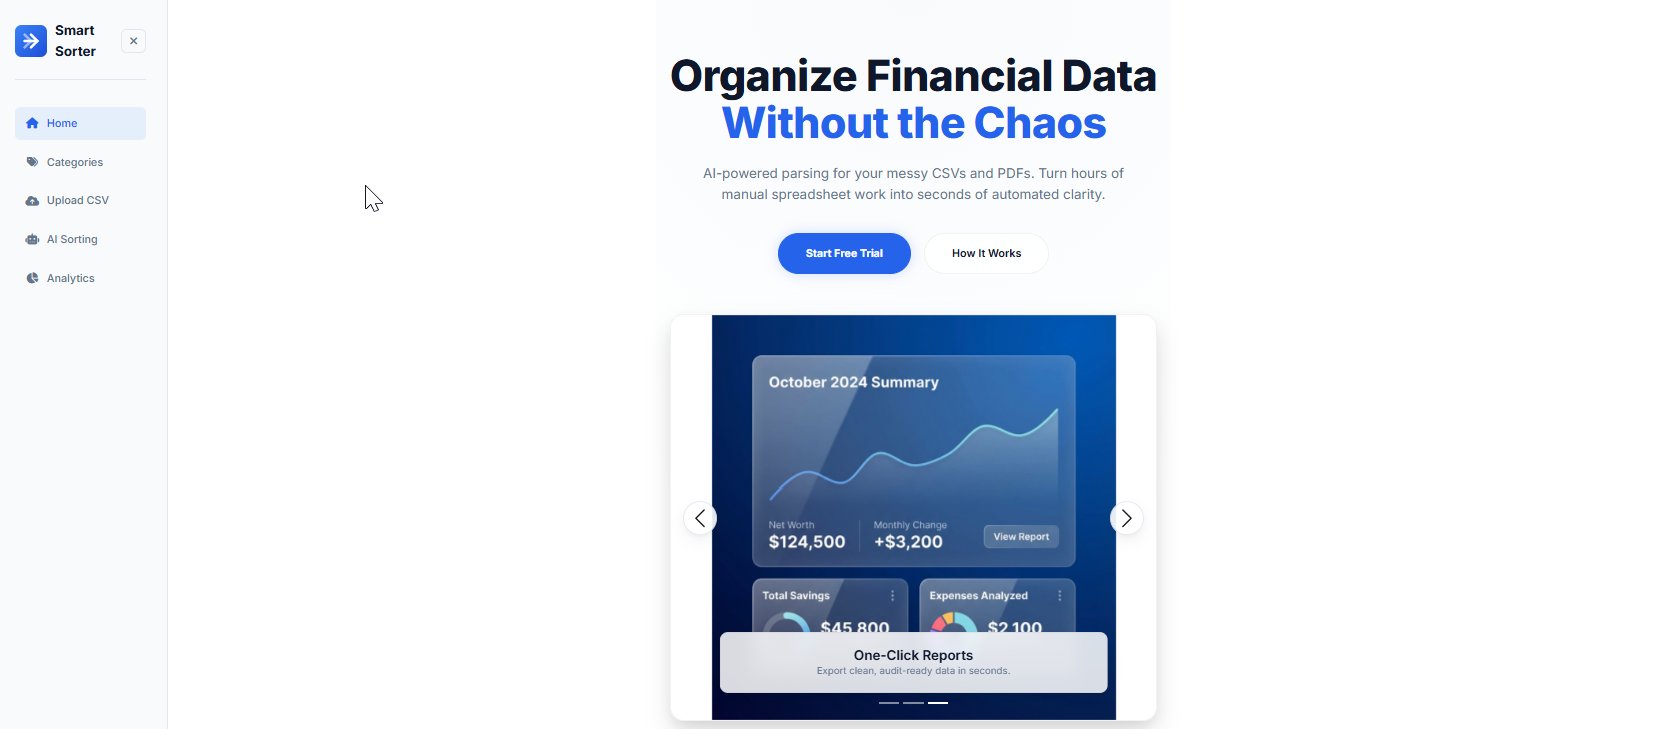
\includegraphics[width=0.8\textwidth]{guide_home.png}
	\caption{Public home page.}
	\label{fig:guide_home}
\end{figure}

\section{Account Registration}
\subsection{Create a New Account}
\begin{normalsteps}
	\item Click \textit{Get Started} from the public navigation menu.
	\item Enter a username.
	\item Enter a valid email address.
	\item Enter a password that satisfies the password rules.
	\item Re-enter the password for confirmation.
	\item Submit the registration form.
	\item After successful signup, continue into the application workflow.
\end{normalsteps}

\begin{figure}[H]
	\centering
	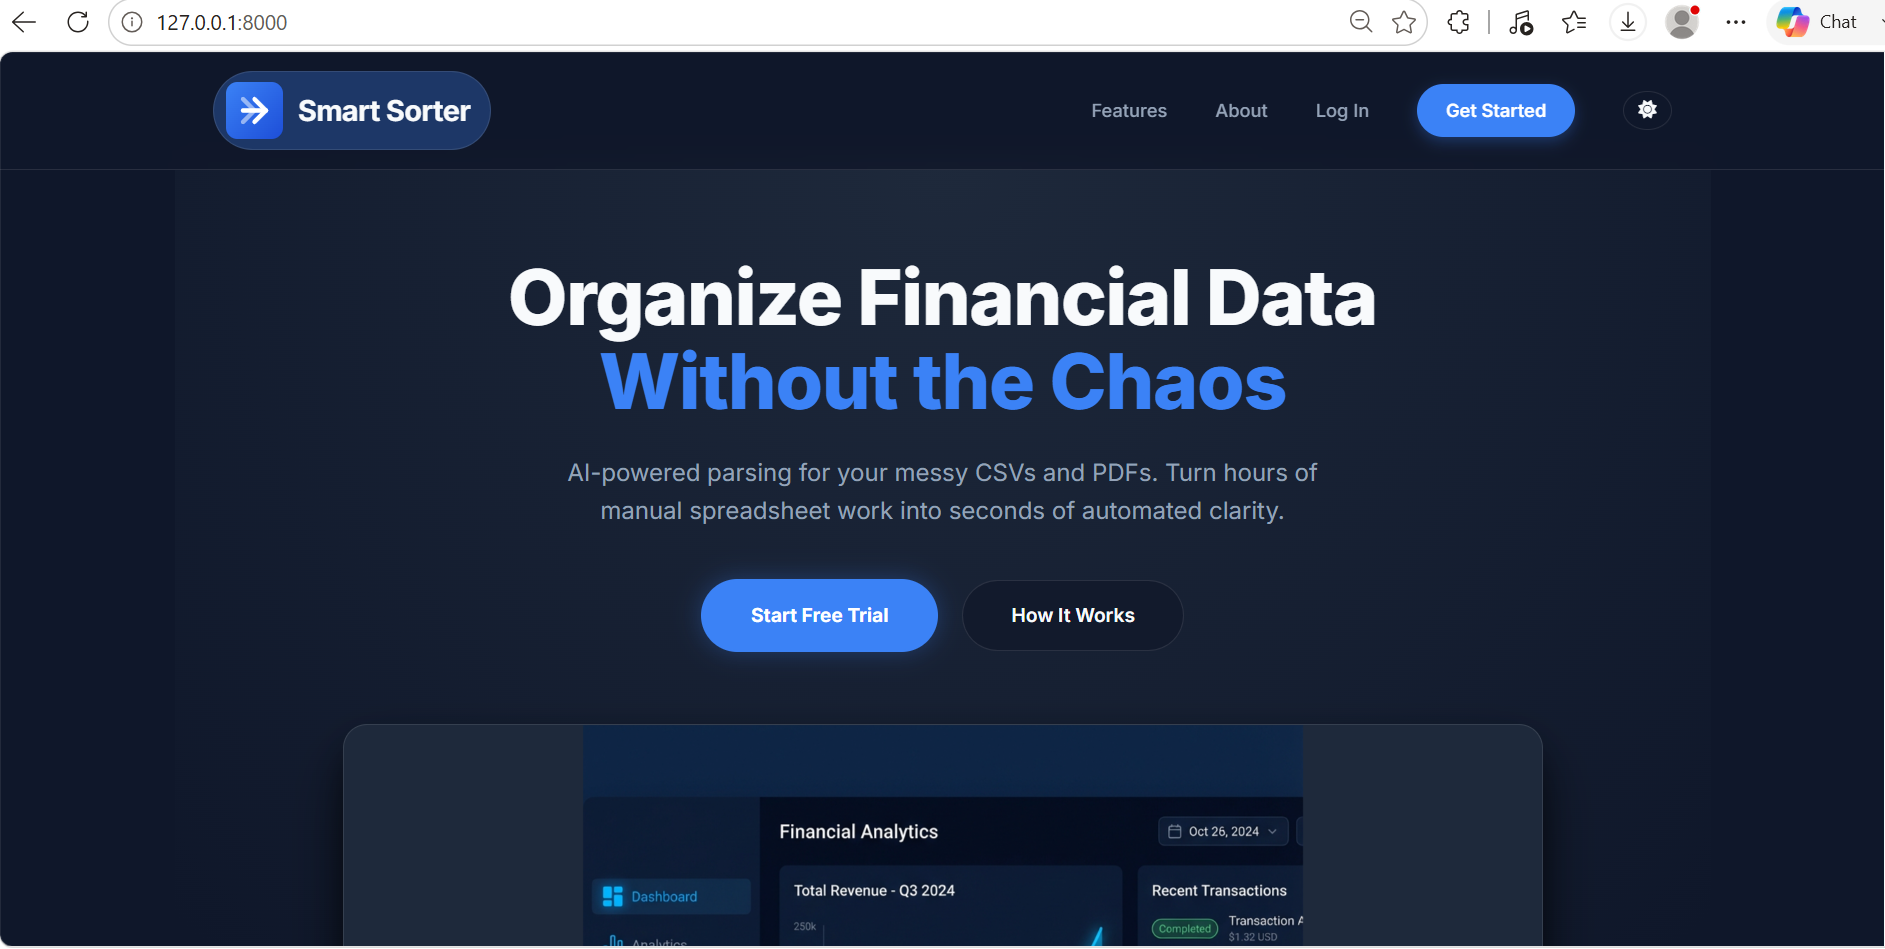
\includegraphics[width=0.8\textwidth]{guide_signup.png}
	\caption{Signup form.}
	\label{fig:guide_signup}
\end{figure}

\subsection{Registration Errors}
\begin{normalsteps}
	\item If the password is too weak, enter a stronger password.
	\item If the password confirmation does not match, re-enter both password fields.
	\item If the username is already taken, choose a different username.
	\item Submit the corrected form.
\end{normalsteps}

\begin{figure}[H]
	\centering
	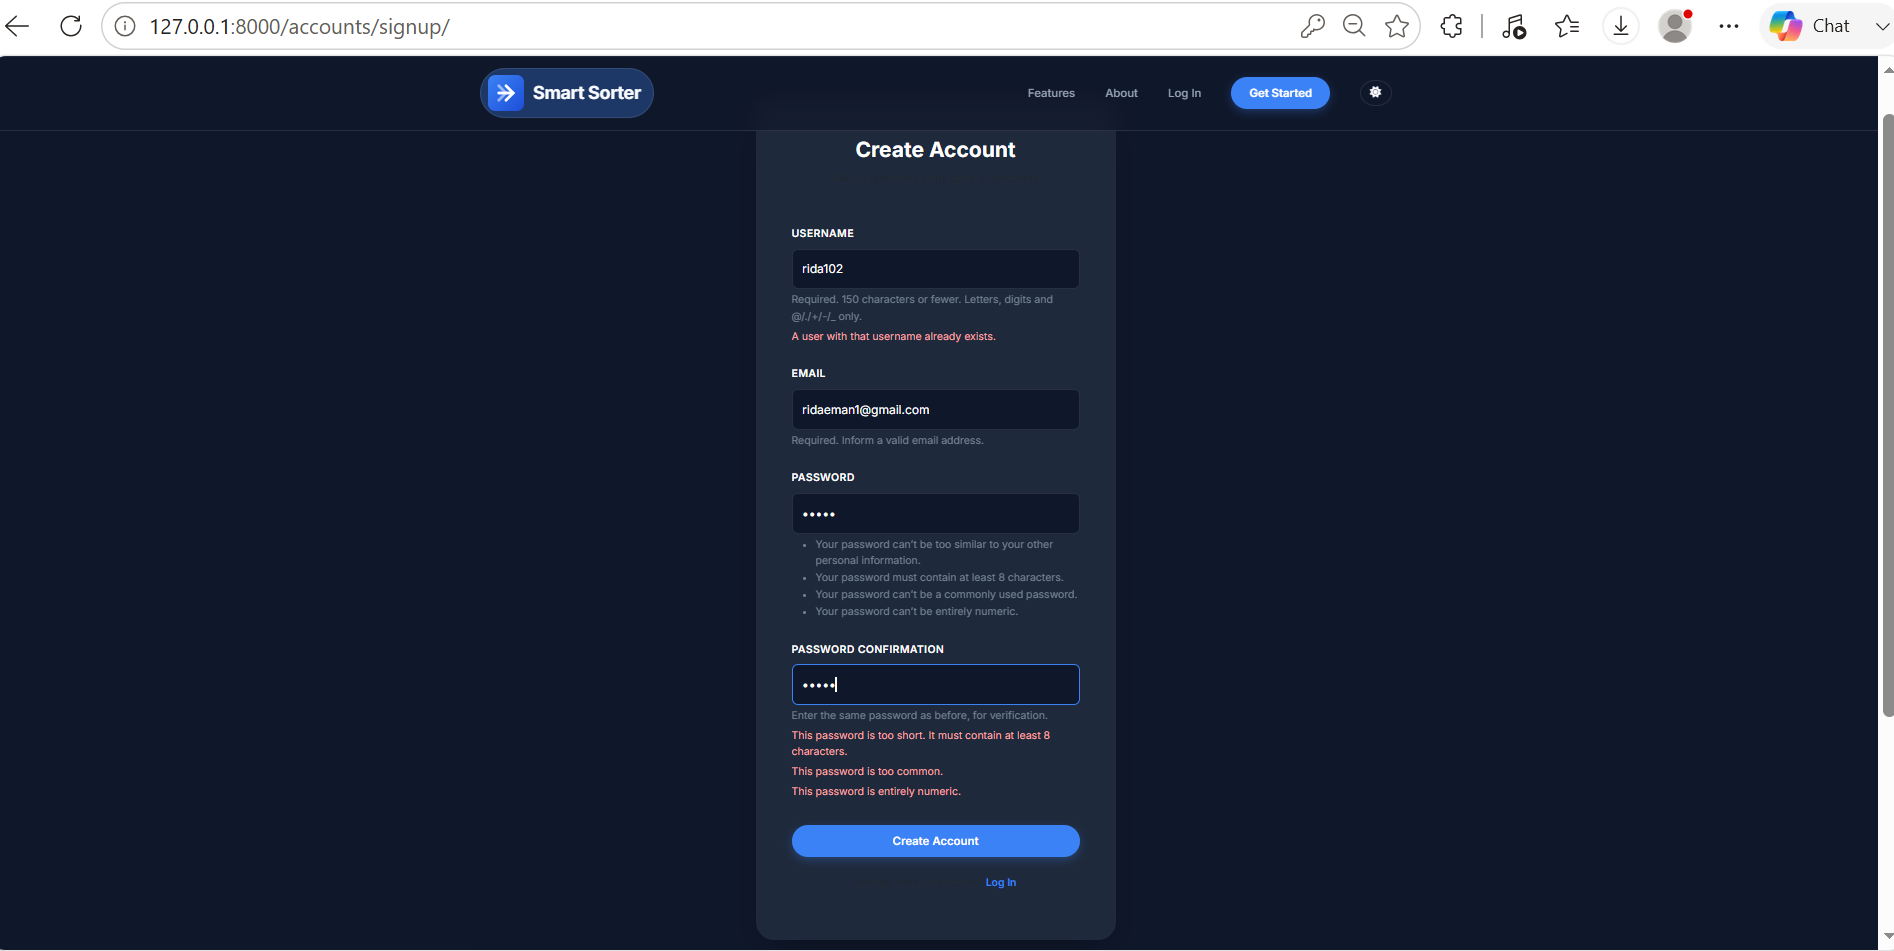
\includegraphics[width=0.8\textwidth]{reg_error.png}
	\caption{Registration error.}
	\label{fig:reg_error}
\end{figure}


\section{Login and Logout}
\subsection{Log In}
\begin{normalsteps}
	\item Click \textit{Log In} from the public navigation menu.
	\item Enter the username.
	\item Enter the password.
	\item Submit the login form.
	\item After successful login, use the sidebar to access Categories, Upload CSV, AI Sorting, and Analytics.
\end{normalsteps}

\begin{figure}[H]
	\centering
	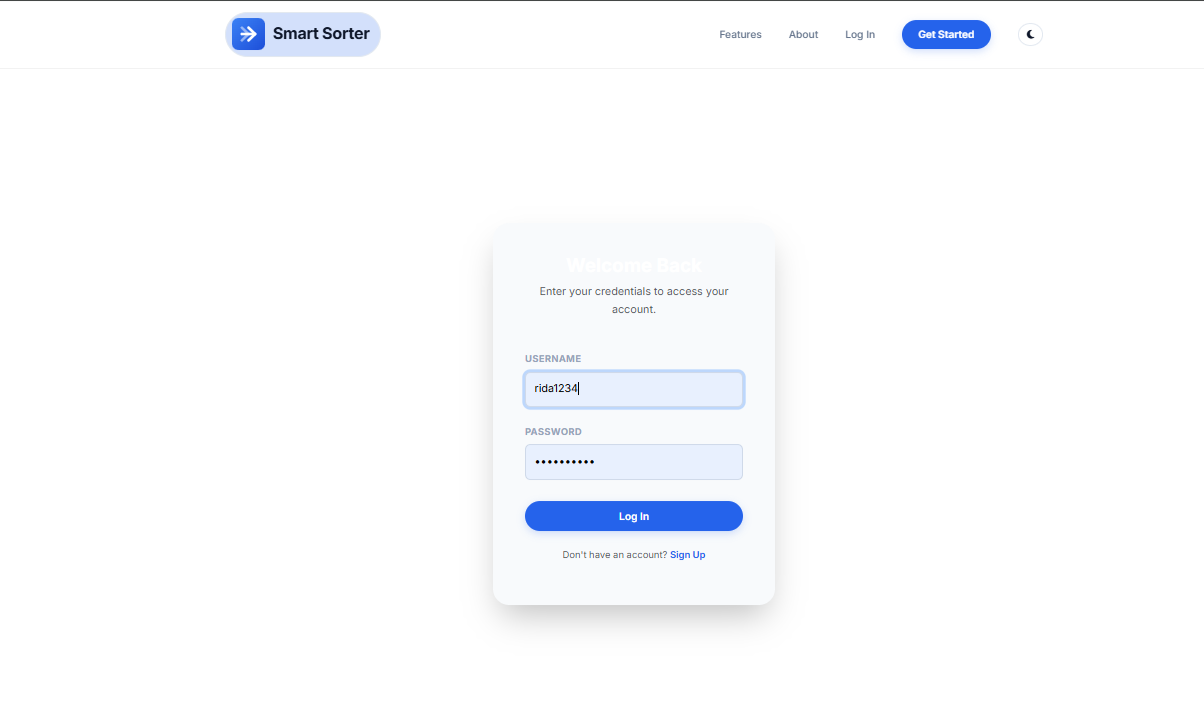
\includegraphics[width=0.8\textwidth]{guide_login.png}
	\caption{Login form.}
	\label{fig:guide_login}
\end{figure}

\subsection{Log Out}
\begin{normalsteps}
	\item Locate the logout button in the authenticated sidebar.
	\item Click \textit{Logout}.
	\item Confirm that the public navigation layout is shown again.
\end{normalsteps}

\section{Category Management}
\subsection{Open Category Management}
\begin{normalsteps}
	\item Log in to the system.
	\item Click \textit{Categories} in the sidebar.
	\item Review the current category list.
	\item Review any quick-add suggestions shown on the page.
\end{normalsteps}

\begin{figure}[H]
	\centering
	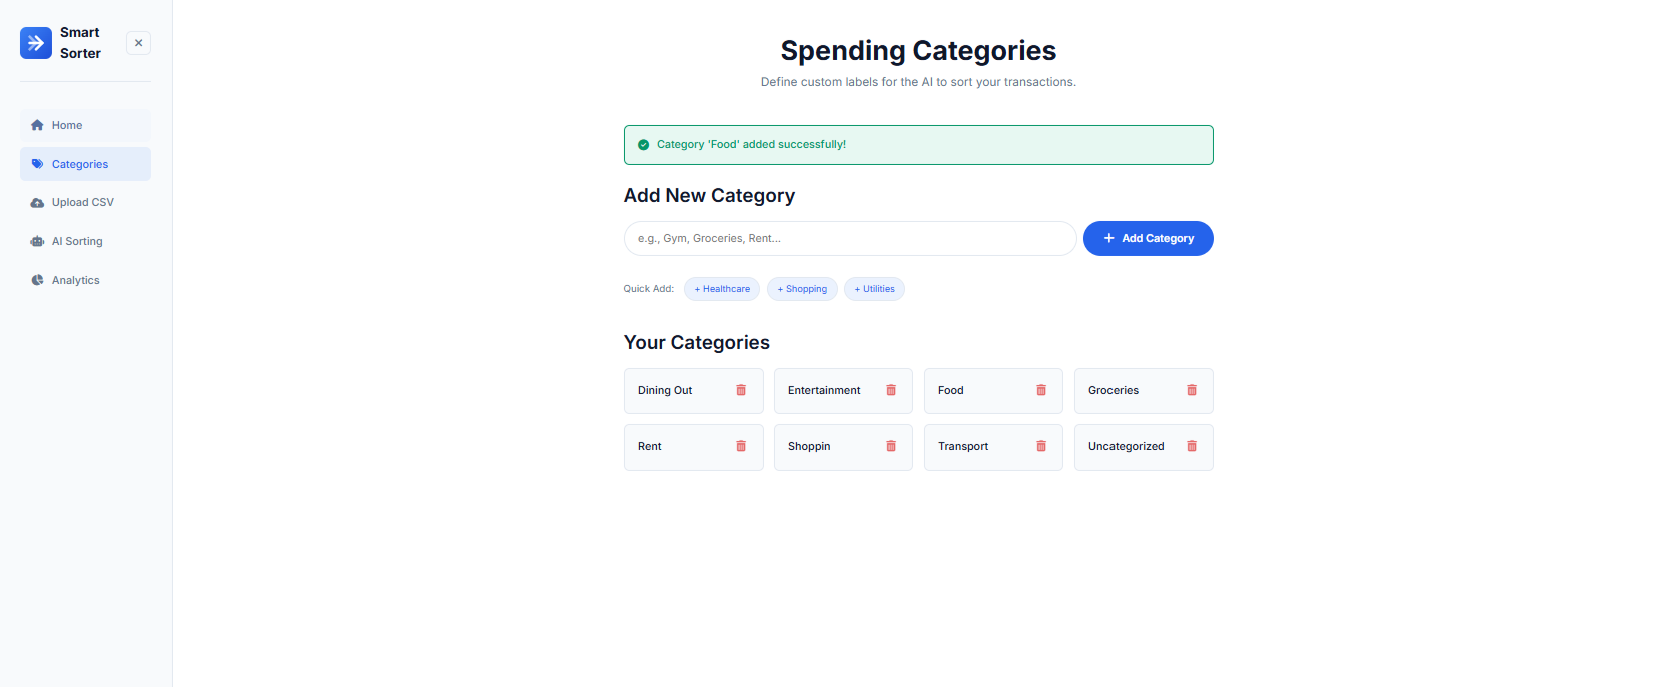
\includegraphics[width=0.8\textwidth]{guide_categories.png}
	\caption{Category management page.}
	\label{fig:guide_categories}
\end{figure}

\subsection{Add a Custom Category}
\begin{normalsteps}
	\item Open the Categories page.
	\item Type the category name in the add category field.
	\item Click \textit{Add Category}.
	\item Confirm that the category appears in the list.
\end{normalsteps}

\subsection{Add a Suggested Category}
\begin{normalsteps}
	\item Open the Categories page.
	\item Locate the quick-add suggestions.
	\item Click the suggestion that should be added to the personal category list.
	\item Confirm that the selected suggestion now appears as a user category.
\end{normalsteps}

\subsection{Delete a Category}
\begin{normalsteps}
	\item Open the Categories page.
	\item Locate the category to remove.
	\item Click the delete button for that category.
	\item Confirm that the category is removed from the list.
\end{normalsteps}

\section{CSV Upload Workflow}
\subsection{Prepare the CSV File}
The CSV file must include the required columns:
\begin{itemize}
	\item \texttt{Date}
	\item \texttt{Description} or \texttt{Raw\_Description}
	\item \texttt{Amount}
\end{itemize}

The file may also include optional columns such as \texttt{Notes}, \texttt{Comments}, \texttt{Merchant\_Name}, \texttt{Merchant}, \texttt{Transaction\_Type}, or \texttt{Type}. Optional columns improve AI classification because they provide more context.

\subsection{Upload Transactions}
\begin{normalsteps}
	\item Log in to the system.
	\item Click \textit{Upload CSV} in the sidebar.
	\item Click the upload zone or drag the CSV file into it.
	\item Confirm that the selected file name appears.
	\item Click \textit{Upload \& Process}.
	\item Wait for the upload to complete.
	\item Review the import success message and transaction preview.
\end{normalsteps}

\begin{figure}[H]
	\centering
	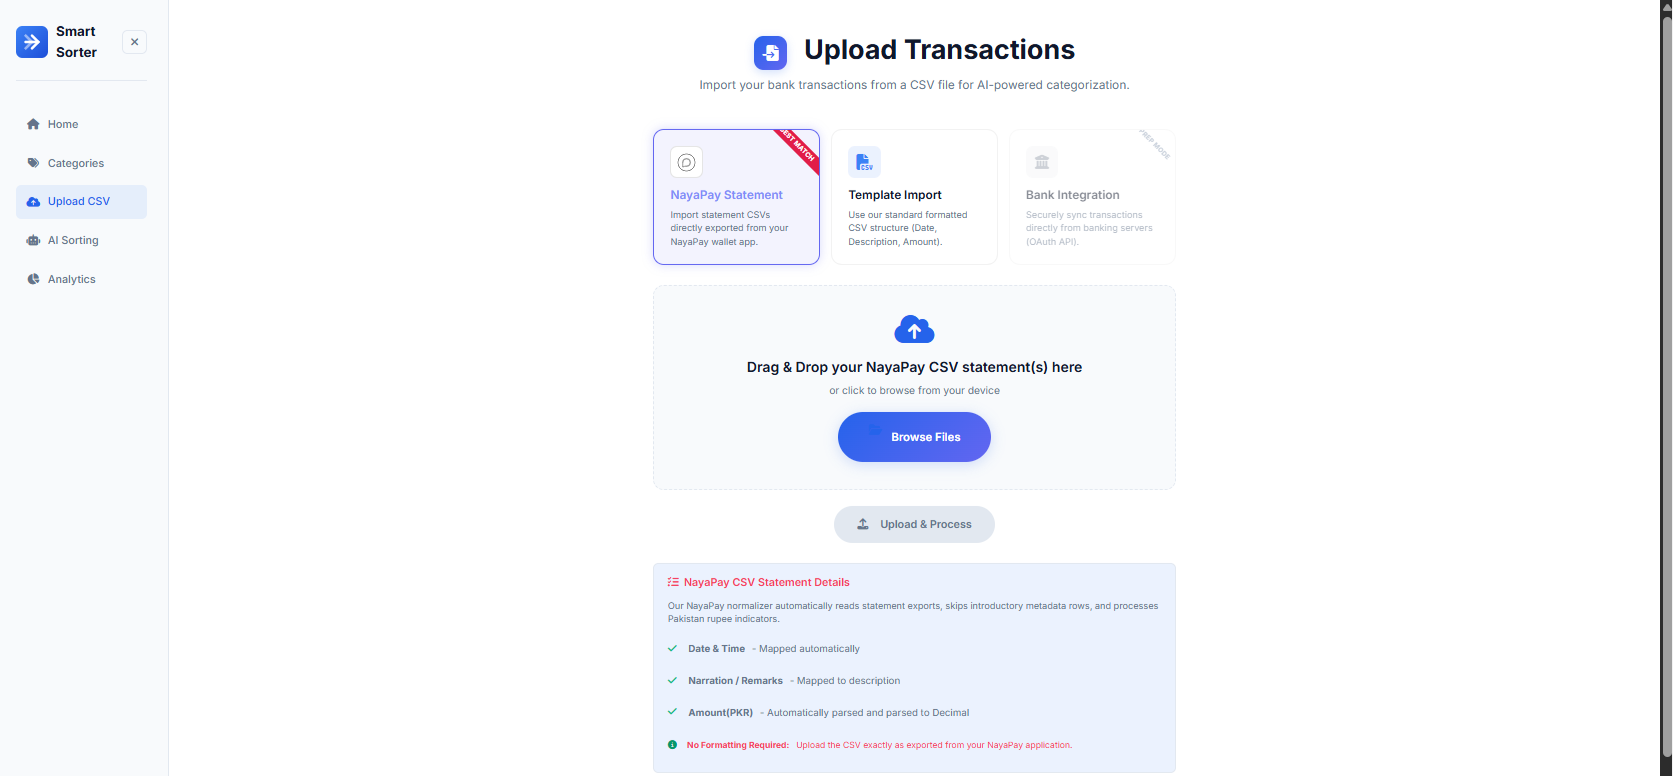
\includegraphics[width=0.8\textwidth]{guide_upload.png}
	\caption{CSV upload page.}
	\label{fig:guide_upload}
\end{figure}

\subsection{Handle Upload Errors}
\begin{normalsteps}
	\item If the system rejects the file type, export or save the source file as CSV.
	\item If a required column is missing, rename or add the required column.
	\item If date rows fail, convert the date values to a supported date format.
	\item If amount rows fail, remove unsupported characters and confirm the value is numeric.
	\item Upload the corrected CSV file again.
\end{normalsteps}

\section{AI Sorting Workflow}
\subsection{Open AI Sorting}
\begin{normalsteps}
	\item Ensure that categories have been created.
	\item Ensure that a CSV file has been uploaded successfully.
	\item Click \textit{AI Sorting} in the sidebar.
	\item Review the Pending, Categorized, Total Transactions, and Categories counters.
\end{normalsteps}

\begin{figure}[H]
	\centering
	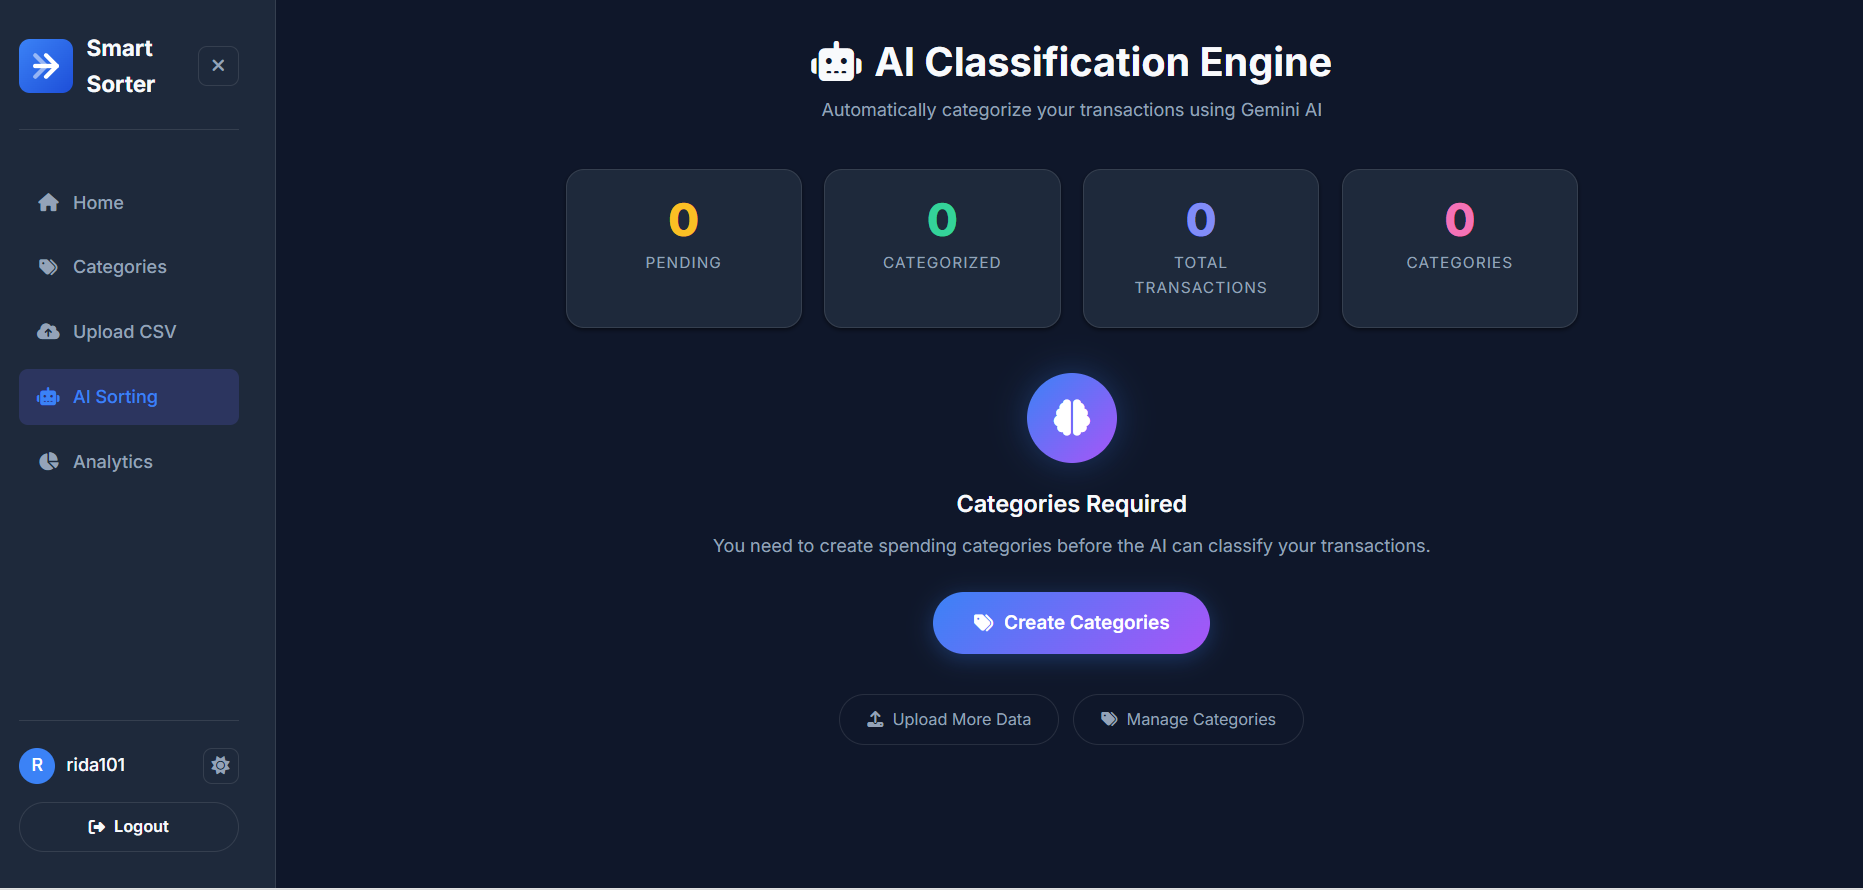
\includegraphics[width=0.8\textwidth]{guide_ai_before.png}
	\caption{AI sorting page before processing.}
	\label{fig:guide_ai_before}
\end{figure}

\subsection{Process Transactions with AI}
\begin{normalsteps}
	\item Open the AI Sorting page.
	\item Confirm that there is at least one pending transaction.
	\item Confirm that there is at least one category.
	\item Click \textit{Process with AI}.
	\item Wait for the processing result.
	\item Review the success, warning, or error messages shown by the system.
	\item Review the classification results table.
\end{normalsteps}

\begin{figure}[H]
	\centering
	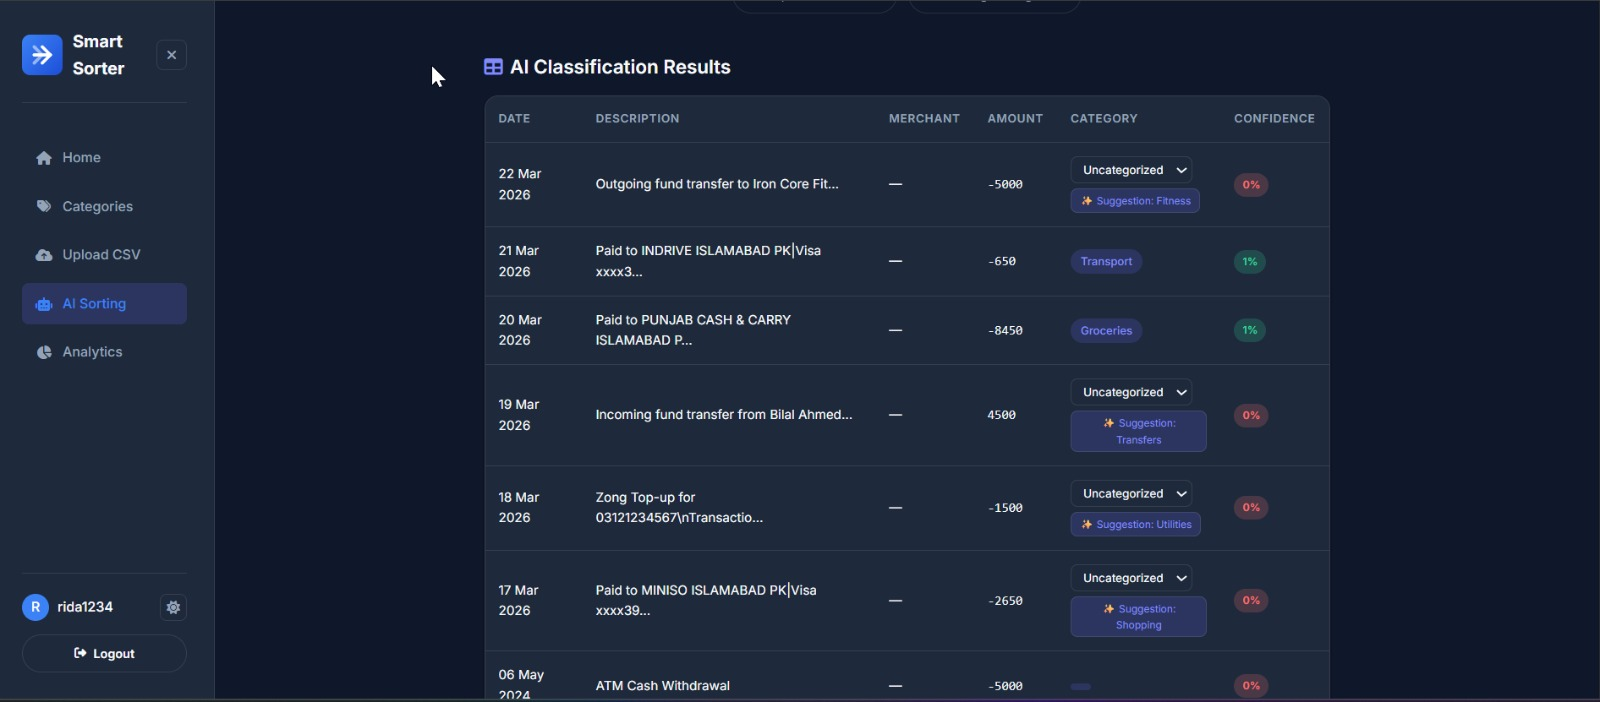
\includegraphics[width=0.8\textwidth]{guide_ai_results.jpeg}
	\caption{AI classification results.}
	\label{fig:guide_ai_results}
\end{figure}

\subsection{If Categories Are Missing}
\begin{normalsteps}
	\item If the AI Sorting page says categories are required, click \textit{Create Categories}.
	\item Add the required category names.
	\item Return to AI Sorting.
	\item Run processing again.
\end{normalsteps}

\subsection{If No Transactions Are Found}
\begin{normalsteps}
	\item If the AI Sorting page says no transactions are found, open Upload CSV.
	\item Upload a valid transaction file.
	\item Return to AI Sorting.
	\item Run processing again.
\end{normalsteps}

\section{Manual Correction Workflow}
\subsection{Correct an Uncategorized Transaction}
\begin{normalsteps}
	\item Open the AI Sorting page after processing.
	\item Locate a transaction marked \textit{Uncategorized}.
	\item Open the category dropdown.
	\item Select the correct category.
	\item Wait for the row to update.
	\item Confirm that the category tag replaces the dropdown.
\end{normalsteps}

\begin{figure}[H]
	\centering
	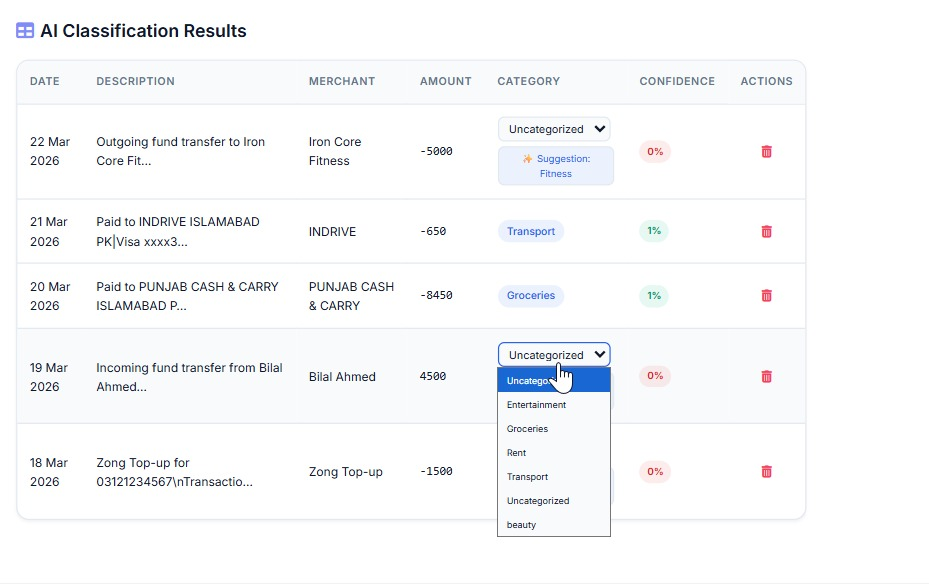
\includegraphics[width=0.8\textwidth]{guide_manual_correction.jpeg}
	\caption{Manual category correction.}
	\label{fig:guide_manual_correction}
\end{figure}

\subsection{Accept an AI Suggestion}
\begin{normalsteps}
	\item Locate an uncategorized transaction that includes an AI suggestion.
	\item Click the suggestion button.
	\item Allow the system to create the category if it does not already exist.
	\item Confirm that the transaction is updated.
\end{normalsteps}

\section{Analytics Dashboard Workflow}
\subsection{Open Analytics}
\begin{normalsteps}
	\item Log in to the system.
	\item Click \textit{Analytics} in the sidebar.
	\item Wait for the Metabase dashboard iframe to load.
	\item Review the available charts and dashboard summaries.
\end{normalsteps}

\begin{figure}[H]
	\centering
	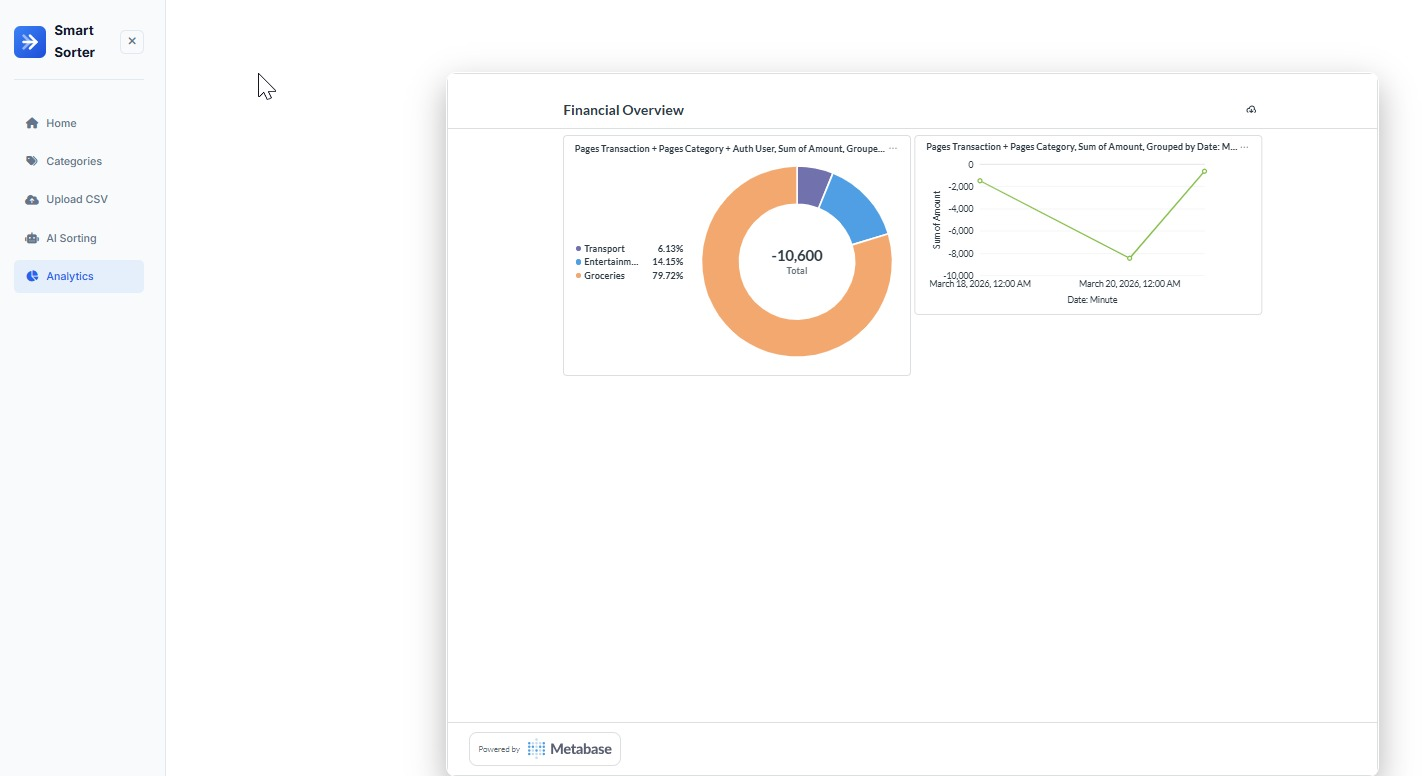
\includegraphics[width=0.8\textwidth]{guide_analytics.jpeg}
	\caption{Embedded Metabase analytics dashboard.}
	\label{fig:guide_analytics}
\end{figure}

\subsection{Handle Analytics Configuration Error}
\begin{normalsteps}
	\item If the analytics page shows a configuration error, contact the system administrator.
	\item The administrator should verify the Metabase site URL.
	\item The administrator should verify the Metabase embedding secret.
	\item The administrator should verify that the dashboard ID exists in Metabase.
	\item Refresh the Analytics page after configuration is corrected.
\end{normalsteps}

\section{Administrator Guide}
\subsection{Access the Admin Panel}
\begin{normalsteps}
	\item Open the admin URL.
	\item Enter administrator credentials.
	\item Submit the login form.
	\item Confirm that the Smart Sorter admin interface loads.
\end{normalsteps}

\begin{figure}[H]
	\centering
	
\includegraphics[width=0.8\textwidth]{guide_admin_login.jpeg}
	\caption{Administrator login page.}
	\label{fig:guide_admin_login}
\end{figure}

\subsection{Manage Default Categories}
\begin{normalsteps}
	\item Log in as administrator.
	\item Open the Default Categories model.
	\item Add common category suggestions such as Groceries, Transport, Utilities, Dining, Shopping, Rent, or Transfers.
	\item Save the default category.
	\item Confirm that the suggestion appears on the user category screen if the user has not already added it.
\end{normalsteps}

\subsection{Review Transactions}
\begin{normalsteps}
	\item Log in as administrator.
	\item Open the Transactions model.
	\item Use filters for user, date, category, AI status, or transaction type.
	\item Use search to locate a description, merchant, username, or note.
	\item Review AI confidence and AI categorization status.
\end{normalsteps}

\begin{figure}[H]
	\centering
	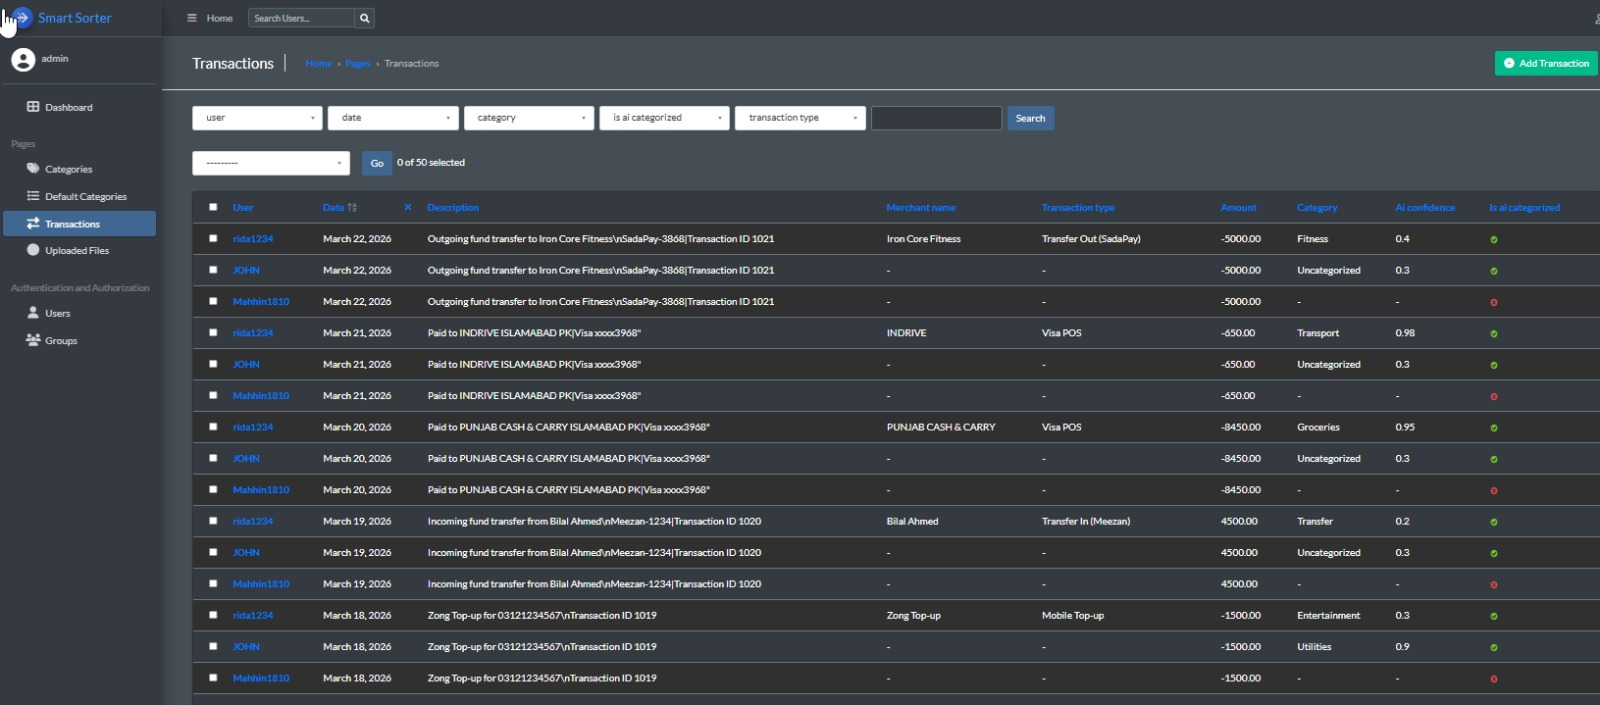
\includegraphics[width=0.8\textwidth]{guide_admin_transactions.jpeg}
	\caption{Transaction records in admin panel.}
	\label{fig:guide_admin_transactions}
\end{figure}

\subsection{Deployment Configuration Checklist}
\begin{normalsteps}
	\item Confirm that PostgreSQL is configured for the final deployment environment.
	\item Confirm that the Gemini API key is available through environment configuration.
	\item Confirm that the Metabase site URL is configured.
	\item Confirm that the Metabase embedding secret is configured.
	\item Confirm that the required Metabase dashboard exists.
	\item Confirm that administrator credentials are protected.
	\item Confirm that debug settings and allowed hosts are appropriate for deployment.
\end{normalsteps}

\section{Recommended User Workflow}
For best results, users should follow the workflow below:
\begin{normalsteps}
	\item Register or log in.
	\item Create a complete category list.
	\item Upload the CSV transaction file.
	\item Review the import preview.
	\item Run AI sorting.
	\item Correct low-confidence or uncategorized rows.
	\item View analytics.
	\item Log out after use.
\end{normalsteps}



    \chapter*{References}
    \addcontentsline{toc}{chapter}{References}
    References will be finalized according to the department's required citation format.

\end{document}
